\chapter{
Estimating the Size of a Closed Population
}
\markboth{Chapter 3}{}
\label{chapt.closed}

\vspace{.3in}

In this chapter we will consider ordinary capture-recapture (CR)
models for estimating population size in closed populations. We will
see that such models are closely related to binomial (or logistic)
regression type models. In fact, when $N$ is known, they are precisely
such models.  We consider some important extensions of ordinary closed
population models that accommodate various types of ``individual
effects'' --- either in the form of explicit covariates (sex, age,
body mass) or unstructured ``heterogeneity'' in the form of an
individual random effect. In general, these models are variations of
generalized linear or generalized linear mixed models (GLMMs).
Because of the paramount importance of this concept, we focus mainly
on fairly simple models in which the observations are individual
encounter frequencies, $y_{i}$ = the number of encounters of
individual $i$ out of $K$ replicate samples of the population which,
for the models we consider here, is the outcome of a binomial random
variable.  Along the way, we consider the spatial context of
capture-recapture data and models and demonstrate that density cannot
be formally estimated when spatial information is ignored. We also
review some of the informal methods of estimating density using CR
methods, and consider some of their limitations.  We will be exposed
to our first primitive spatial capture-recapture models which arise as
relatively minor variations of so-called ``individual covariate
models'' (of the \citet{huggins:1989} and \citet{alho:1990}
variety). In a sense, the point of this chapter is to establish that
linkage in a direct and concise manner beginning with the basic
``Model M0'' and extensions of that model to include individual
heterogeneity and also individual covariates. A special type of
individual covariate models is distance sampling, which could be
thought of as the most primitive spatial capture-recapture model.  In
later chapters we further develop and extend ideas introduced in this
chapter.

We emphasize Bayesian analysis of capture-recapture models and we
accomplish this using a method related to classical ``data
augmentation'' from the statistics literature
\citet[e.g.,][]{tanner_wong:1987}).  This is a general concept in
statistics but, in the context of capture-recapture models where $N$
is unknown, it has a consistent implementation across classes of
capture-recapture models and one that is really convenient from the
standpoint of doing MCMC \citep{royle_etal:2007}. We use data
augmentation throughout this book and thus emphasize its conceptual
and technical origins and demonstrate applications to closed
population models.  We refer the reader to
\citet[][ch. 6]{kery_schaub:2011} for an accessible and complimentary
development of ordinary closed population models.


\section{The Simplest Closed Population Model: Model M0}

We suppose that there exists a population of $N$ individuals which we
subject to repeated sampling, say over $K$ nights, where individuals
are captured, marked, and subsequently recaptured.  We suppose that
individual encounter histories are obtained, and these are of the form
of a sequence of 0's and 1's indicating capture $(y=1)$ or not $(y=0)$
during any sampling occasion (``sample'').  As an example, suppose
$K=5$ sampling occasions, then an individual captured during sample 2
and 3 but not otherwise would have an encounter history of the form
${\bf y}=(0,1,1,0,0)$. Thus, the observation ${\bf y}_{i}$ for each
individual $(i)$ is a vector having elements denoted by $y_{ik}$ for
$k=1,2,..,K$. Usually this is organized as a row of a matrix with
elements $y_{ik}$, see Table \ref{tab.3.1}.  Except where noted
explicitly, we suppose that observations are independent within
individuals and among individuals.  Formally, this allows us to say
that $y_{ik}$ are Bernoulli random variables and we may write $y_{ik}
\sim \mbox{Bern}(p)$.  Consequently, for this very simple model in
which $p$ is in fact constant, then we can declare that the individual
encounter frequencies (total captures), $y_{i} = \sum_{k} y_{ik}$,
have a binomial distribution based on a sample of size $K$. That is
\[
y_{i}  = \sum_{k} y_{ik} \sim \mbox{Bin}(p,K)
\]
for every individual in the population. This is a remarkably simple
model that forms the cornerstone of almost all of classical
capture-recapture models, including most spatial capture-recapture
models discussed throughout this book.  Evidently, the basic
capture-recapture model structure is precisely a simplistic version of
a logistic-regression model with only an intercept term
($\mbox{logit}(p) = \mbox{constant}$).  To say that all
capture-recapture models are just logistic regressions is only
slightly inaccurate. In fact, we are proceeding here ``conditional on
$N$'', i.e., as if we knew $N$. In practice we don't, of course, and
that is kind of the point of capture-recapture models as estimating
$N$ is the central objective. But, by proceeding conditional on $N$,
we can specify a simple model and then deal with the fact that $N$ is
unknown using standard methods that you are already familiar with
(i.e., GLMs - see chapter 2).
\begin{table}
\centering
\caption{a capture-recapture data set with $n=6$ observed individuals
and $K=5$ samples.}
\begin{tabular}{r|ccccc|c}
&  \multicolumn{5}{c}{Sample occasion} &  \\ \hline
 indiv $i$ &  1 & 2 & 3 & 4 & 5 & $y_{i}$ \\ \hline
  1 &     1 & 0 & 0 & 1 & 0  & 2   \\
  2 &     0 & 1 & 0 & 0 & 1  & 2   \\
  3 &     1 & 0 & 0 & 1 & 0  & 2   \\
  4 &     1 & 0 & 1 & 0 & 1  & 3   \\
  5 &     0 & 1 & 0 & 0 & 0  & 1   \\
  $n=6$ & 1 & 0 & 0 & 0 & 0  & 1   \\ \hline
\end{tabular}
\label{tab.3.1}
\end{table}

Assuming individuals of the population are observed independently, the
joint probability distribution of the observations is the product of
$N$ binomials
\begin{eqnarray*}
  \Pr(y_1, \ldots, y_N | p) &=& \prod_{i=1}^N  \mathrm{Bin}(y_i | K, p) \\
   &=& \prod_{k=0}^K  \pi(k)^{n_k}
\end{eqnarray*}
where $\pi(k) = \mathrm{Bin}(k | K,p)$ and where $n_k = \sum_{i=1}^N
I(y_i = k)$ denotes the number of individuals captured $k$ times in
$K$ surveys. We emphasize that this is conditional on $N$, in which
case we get to observe the $y=0$ observations and the resulting data
are just $iid$ binomial counts. Because this is a binomial regression
model of the variety described in chapter 2, fitting this model using
a BUGS engine poses no difficulty.

The essential problem in capture-recapture, however, is that $N$ is
not known because the number of uncaptured/missing individuals (i.e.,
those in the zero cell that occur with probability $\pi(0)$) is
unknown.  Consequently, the observed capture frequencies $n_k$ are no
longer independent. Instead, their joint distribution is multinomial
(e.g., see \citet[][p. xyz]{illian_etal:2008}):
\begin{equation}
\label{eq:multinomialForM0}
    n_1, n_2, \ldots, n_K \sim \mathrm{Multin}(N, \pi(1), \pi(2), \ldots, \pi(K))
\end{equation}
Note that in our notation the number of uncaptured/missing individuals is
denoted by $n_0 = N - n$, where $n = \sum_{k=1}^K n_k$ denotes the total
number of distinct individuals seen in the $K$ samples.

To fit the model in which $N$ is {\it unknown}, we can regard $N$ as a
parameter and maximize the multinomial likelihood directly.  While
direct likelihood analysis of the multinomial model is
straightforward, that does not prove to be too useful in practice
because we seldom are concerned with models for the aggregated
encounter history frequencies. In many instances, including for
spatial capture-recapture (SCR) models, we require a formulation of
the model that can accommodate individual level covariates which we
address subsequently in this chapter.



\subsection{The Spatial Context of Capture-Recapture}

A common assumption made is that of population ``closure'' which is
really just a colloquial way of saying (in part) the Bernoulli
assumptions stated explicitly above. In the biological context,
closure means, strictly, no additions or subtractions from the
population during study. This is manifest by the statement that the
encounters are independent and identically distributed (iid) Bernoulli
trials.  In practice, closure is usually interpreted by the manner in
which potential violations of that assumption arise. In particular,
two important elements of the closure assumption are ``demographic''
and ``geographic'' closure. If an individual dies then subsequent
values of $y_{ik}$ are clearly no longer Bernoulli trials with the
same parameter $p$. If there is no mortality or recruitment in the
population, then we say that demographic closure is
satisfied. Similarly, animals may emigrate or immigrate. If they do
not, then geographic closure is satisfied. Sometimes a distinction is
made between temporary and permanent emigration or immigration. That
is a relevant distinction in spatial capture-recapture models, because
SCR models explicitly accommodate ``temporary emigration'' of a
certain type, due to individuals moving about their home range. The
demographic closure assumption can also be relaxed using SCR models,
but we will save that discussion for chapter \ref{chapt.scr0}.


\subsection{Conditional likelihood}

We saw that a basic closed population model is a simple logistic
regression model if $N$ is known and, when $N$ is unknown, the model
is multinomial with index or sample size parameter $N$. This
multinomial model, being conditional on $N$, is sometimes referred to
as the ``joint likelihood'' the ``full likelihood'' or the
``unconditional likelihood'' (or model in place of likelihood). This
formulation differs from the so-called ``conditional likelihood''
approach in which the likelihood of the observed encounter histories
is devised conditional on the event that an individual is captured at
least once.  To construct this likelihood, we have to recognize that
individuals appear or not in the sample based on the value of the
random variable $y_{i}$, that is, we capture them if and only if
$y_{i}>0$.  The observation model is therefore based on $\Pr(y|y>0)$.
For the simple case of Model M0, the resulting conditional
distribution is a ``zero truncated'' binomial distribution which
accounts for the fact that we cannot observe the value $y=0$ in the
data set \citep[see][section XYZ]{royle_dorazio:2008}.  Both the
conditional or unconditional models are legitimate modes of analysis
in all capture-recapture types of studies, and they provide equally
valid descriptions of the data and for many practical purposes provide
equivalent inferences, at least in large sample sizes
\citep{sanathanan:1972}.

In this book we emphasize Bayesian analysis of capture-recapture
models using data augmentation (discussed subsequently), which
produces yet a third distinct formulation of capture recapture-models
based on the zero-{\it inflated} binomial distribution that we
describe in the next section.  Thus, there are 3 distinct formulations
of the model -- or models of analysis -- for analyzing all
capture-recapture models based on the (1) binomial model for the joint
or unconditional specification; (2) zero-truncated binomial that
arises ``conditional on $n$''; and (3) the zero-inflated binomial that
arises under data augmentation.  Each formulation has a distinct
complement of model parameters (shown in Table \ref{tab.3.modes} for
Model M0).


\begin{table}
\centering
\begin{tabular}{ccc}
Mode of analysis & parameters in model & statistical model \\ \hline
Joint likelihood                &	$p$, $N$	&	multinomial with index $N$\\
Conditional likelihood 		&	$p$	&	zero-truncated binomial \\
Data augmentation		&	$p$, $\psi$	&	zero-inflated binomial\\
\end{tabular}
\caption{Modes of analysis of capture-recapture models.}
\label{tab.3.modes}
\end{table}



\section{ Data Augmentation }

We consider a method of analyzing closed population models using data
augmentation (DA) which is useful for Bayesian analysis and, in
particular, analysis of models using the various BUGS engines and
other software.  Data augmentation is a general statistical concept
that is widely used in statistics in many different settings. The
classical reference is \citet{tanner_wong:1987} but see also
\citet{liu_wu:1999}.  Data augmentation can be adapted to provide a
very generic framework for Bayesian analysis of capture-recapture
models with unknown $N$. This idea was introduced for closed
populations by \citet{royle_etal:2007}, and has subsequently been
applied to a number of different contexts including individual
covariate models \citep{royle:2009}, open population models
\citep{royle_dorazio:2008,royle_dorazio:2010, gardner_etal:2010},
spatial capture-recapture models \citep{royle_young:2008,
  royle_etal:2010, gardner_etal:2009}, and many others.


Conceptually, data augmentation takes the data you wish you
had - that is, the data set with $N$ rows - the known-$N$ data set - and
embeds that data set into a larger data set having $M > N$ rows.
\footnote{ RC: Might be just me, but I find that formulation a little
confusing... I think it's the 'data you wish you had because that's
effectively data you don't have. I think it might be easier to grasp
if this were explained with the data you do have - based on n. }
 It is always possible, in practice, to choose $M$ pretty easily for
 a given problem and context. Then, under data augmentation, analysis
 is focused on the ``augmented data set.'' That is, we analyze the bigger
 data set - the one having $M$ rows - with an appropriate model that
 accounts for the augmentation. Inference is focused directly on
 estimating the proportion $\psi = E[N]/M$, instead of directly on $N$,
 where $\psi$ is the ``data augmentation parameter.''


\subsection{DA links occupancy models and closed population models}

We provide a heuristic description of data augmentation based on the
close correspondence between so-called ``occupancy'' models and closed
population models following \citet[][sec. xyz]{royle_dorazio:2008}.

In occupancy models \citep{mackenzie_etal:2002, tyre_etal:2003} the
sampling situation is that $M$ sites, or patches, are sampled multiple
times to assess whether a species occurs at each site.  This yields
encounter data such as that illustrated in the left panel of Table
\ref{closed.tab.occ}. The important problem is that a species may occur at
a site, but go undetected, yielding the ``all-zero'' encounter
histories which are observed. However, some of the all-zeros may well
correspond to sites where the species in fact {\it does not}
occur. Thus, while the zeros are observed, there are too many of them
and, in a sense, the inference problem is to allocate the zeros into
``structural'' (fixed) and ``sampling'' (or stochastic) zeros. More
formally, inference is focused on the parameter $\psi$, the
probability that a site is occupied.  In contrast, in classical closed
population studies, we observe a data set as in the middle panel of
Table \ref{closed.tab.occ} where {\it no} zeros are observed. The inference
problem is, essentially, to estimate how many sampling zeros there are
- or should be - in a ``complete'' data set. The inference objective
(how many sampling zeros?) is precisely the same for both types of
problems if an upper limit $M$ is specified for the closed population
model. The only distinction being that, in occupancy models, $M$ is
set by design (i.e., the number of sites to visit) whereas a natural
choice of $M$ for capture-recapture models may not be
obvious. However, by assuming a uniform prior for $N$ on the integers
$[0,M]$, this upper bound is induced \citep{royle_etal:2007}. Then,
one can analyze capture-recapture models by adding $M-n$ all-zero
encounter histories to the data set and regarding the augmented data
set, essentially, as a site-occupancy data set.

Thus, the heuristic motivation of data augmentation is to fix the size
of the data set by adding {\it too many} all-zero encounter histories
to create the data set shown in the right panel of Table
\ref{closed.tab.occ} - and then analyze the augmented data set using an
occupancy type model which includes both ``unoccupied sites'' as well
as ``occupied sites'' at which detections did not occur. We call these
$M-n$ all-zero histories ``potential individuals'' because they exist
to be recruited (in a non-biological sense) into the population, for
example during an analysis by MCMC.

To analyze the augmented data set, we recognize that it is a
zero-inflated version of the known-$N$ data set. That is, some of the
augmented all-zeros are sampling zeros (corresponding to actual
individuals that were missed) and some are ``structural'' zeros, which
do not correspond to individuals in the population. For a basic
closed-population model, the resulting likelihood under data
augmentation - that is, for the data set of size $M$ -- is a simple
zero-inflated binomial likelihood.  The zero-inflated binomial model
can be described ``hierarchically'', by introducing a set of binary
latent variables, $z_{1},z_{2},\ldots, z_{M}$, to indicate whether
each individual $i$ is ($z_i=1$) or is not ($z_i=0$) a member of the
population of $N$ individuals exposed to sampling. We assume that
$z_{i} \sim \mbox{Bern}(\psi)$ where $\psi$ is the probability that an
individual in the data set of size $M$ is a member of the sampled
population - in the sense that $1-\psi$ is the probability of
realizing a ``structural zero'' in the augmented data set.  The
zero-inflated binomial model which arises under data augmentation can
be formally expressed bythe following set of assumptions:

\begin{eqnarray*}
 y_{i}|{z_{i}=1} & \sim  &\mbox{Bin}(K, p) \\
 y_{i}|{z_{i}=0} & \sim &  \delta(0)  \\
 z_{i} & \stackrel{iid}{\sim} & \mbox{Bern}(\psi) \\
 \psi & \sim & \mathrm{Unif}(0,1) \\
 p & \sim & \mathrm{Unif}(0,1)
\end{eqnarray*}
for $i=1, \ldots, M$, where $\delta(0)$ is a point mass at $y=0$.

We note that $N$ is no longer an explicit parameter of this
model. Instead, we estimate $\psi$ and functions of the latent
variables. In particular, under the assumptions of the zero-inflated
model, $z_{i} \stackrel{iid}{\sim} \mbox{Bern}(\psi)$; therefore, $N$
is a function of these latent variables:
 \[
 N = \sum_{i=1}^{M} z_{i}.
\]
Further, we note that the latent $z_i$ parameters can be removed from
the model by integration, in which case the joint probability of the
data is
\begin{equation}
  \Pr(y_1, \ldots, y_M | p, \psi) = \prod_{i=1}^M  \psi \mathrm{Bin}(y_i | K, p) +  I(y_i=0) (1-\psi)
\end{equation}
Which can be maximized directly to obtain the MLEs of the structural
parameters $\psi$ and $p$ or those of other more complex models
\citep[e.g., see][]{royle:2006}. We could estimate these parameters
and then use them to obtain an estimator of $N$ using the so-called
``Best unbiased predictor'' \citep[see][]{royle_dorazio:2011}.

\begin{table}
\centering
\caption{Hypothetical occupancy data set (left), capture-recapture data
 in standard form (center), and capture-recapture data augmented with
 all-zero capture histories (right). }
\begin{tabular}{cccc|cccc|cccc}
\hline
\multicolumn{4}{c}{Occupancy data}    &
\multicolumn{4}{c}{Capture-recapture} &
\multicolumn{4}{c}{Augmented C-R}     \\ \hline
site    & k=1 & k=2 & k=3 & ind & k=1 &k=2  & k=3 & ind & k=1 & k=2 & k=3           \\ \hline
1  & 0   & 1   & 0   & 1   & 0   & 1  & 0   & 1   & 0   & 1   & 0                   \\
2  & 1   & 0   & 1   & 2   & 1   & 0 & 1    & 2 & 1 & 0 & 1 \\
3  & 0   & 1   & 0   & .   & 0   & 1 & 0    & 3 & 1 & 0 & 1 \\
4  & 1   & 0   & 1   & .   & 1   & 0 & 1    & 4 & 1 & 0 & 1 \\
5  & 0   & 1   & 1   & .   & 0   & 1 & 1    & 5 & 1 & 0 & 1 \\
.  & 0   & 1   & 1   & .   & 0   & 1 & 1    & . & 0 & 1 & 1 \\
.  & 1   & 1   & 1   & .   & 1   & 1 & 1    & . & 0 & 1 & 1 \\
.  & 1   & 1   & 1   & .   & 1   & 1 & 1    & . & 1 & 1 & 1 \\
   & 1   & 1   & 1   & .   & 1   & 1 & 1    & . & 1 & 1 & 1 \\
n  & 1   & 1   & 1   & n   & 1   & 1 & 1    & n & 1 & 1 & 1 \\
.  & 0   & 0   & 0   &     &     &   &      & . & 0 & 0 & 0 \\
.  & 0   & 0   & 0   &     &     &   &      & . & 0 & 0 & 0 \\
   & 0   & 0   & 0   &     &     &   &      &   & 0 & 0 & 0 \\
   & 0   & 0   & 0   &     &     &   &      &   & 0 & 0 & 0 \\
   & 0   & 0   & 0   &     &     &   &      &   & 0 & 0 & 0 \\
   & 0   & 0   & 0   &     &     &   &      & N & 0 & 0 & 0 \\
.  & 0   & 0   & 0   &     &     &   &      & . & 0 & 0 & 0 \\
.  & 0   & 0   & 0   &     &     &   &      &   & 0 & 0 & 0 \\
M  & 0   & 0   & 0   &     &     &   &      & . & 0 & 0 & 0 \\
   &     &     &     &     &     &   &      & . & . & . & . \\
   &     &     &     &     &     &   &      & . & . & . & . \\
   &     &     &     &     &     &   &      & . & . & . & . \\
   &     &     &     &     &     &   &      & M & 0 & 0 & 0 \\
\end{tabular}
\label{closed.tab.occ}
\end{table}


\subsection{Model $M_0$ in BUGS}

For model $M_0$ in which we can aggregate the encounter data to
individual-specific encounter frequencies, the augmented data are
given by the vector of frequencies $(y_{1}, \ldots, y_{n}, 0, 0,
\ldots, 0)$. The zero-inflated model of the augmented data combines
the model of the latent variables, $z_{i} \sim \mbox{Bern}(\psi)$ with
the conditional-on-$z$ binomial model:
\begin{eqnarray*}
y_{i} | z_{i} = 0 &\sim& \delta(0) \\
y_{i}|z_{i} = 1   &\sim& \mbox{Bin}(K,p)
\end{eqnarray*}
It is convenient to express the conditional-on-$z$ observation model concisely as:
\[
 y_{i}|z_{i} \sim \mbox{Bin}(K, p z_{i})
\]
Thus, if $z_{i}=0$ then the success probability of the binomial
distribution is identically 0 whereas, if $z_{i}=1$, then the success
probability is $p$. This is useful in describing the model in the {\bf
  BUGS}
language, as shown below. Note the last line of the model
specification here provides the expression for computing $N$ from the
data augmentation variables $z_{i}$.
{\small
\begin{verbatim}
p  ~ dunif(0,1)
psi~dunif(0,1)

# nind = number of individuals captured at least once
#   nz = number of uncaptured individuals added for PX-DA
for(i in 1:(nind+nz)) {
    z[i]~dbern(psi)
   mu[i]<-z[i]*p
    y[i]~dbin(mu[i],K)
 }

N<-sum(z[1:(nind+nz)])
\end{verbatim}
}


Specification of a more general model in terms of the individual
encounter observations $y_{ik}$ is not much more difficult than for
the individual encounter frequencies.  We define the
observation model by a double loop and change the indexing of things
accordingly, i.e.,
\begin{verbatim}
for(i in 1:(nind+nz)) {
    z[i]~dbern(psi)
  for(k in 1:K){
      mu[i,k]<-z[i]*p
      y[i,k]~dbin(mu[i,k],1)
  }
}
\end{verbatim}
In this manner, it is straightforward to incorporate covariates on $p$
(see discussion of this below and also chapt. 8 (REF XYZ) and consider
other extensions.


\subsection{Formal development of data augmentation}

Use of DA for solving inference problems with unknown $N$ can be
justified as originating from the choice of uniform prior on $N$.  The
$\mathrm{Unif}(0,M)$ prior for $N$ is innocuous in the sense that the
posterior associated with this prior is equal to the likelihood for
sufficiently large $M$.  One way of inducing the $\mathrm{Unif}(0,M)$
prior on $N$ is by assuming the following hierarchical prior:
\begin{eqnarray}\label{eq:NgivenM}
  N &\sim& \mathrm{Bin}(M, \psi) \\ \nonumber
  \psi &\sim& \mathrm{Unif}(0,1)
\end{eqnarray}
which includes a new model parameter $\psi$.  This parameter denotes
the probability that an individual in the super-population of size $M$
is a member of the population of $N$ individuals exposed to sampling.
The model assumptions, specifically the multinomial model (eq. XYZ)
and eq. \ref{eq:NgivenM}, may be combined to yield a
reparameterization of the conventional model that is appropriate for
the augmented data set of known size $M$:
\begin{equation}\label{eq:multinomialForDA}
    (n_1, n_2, \ldots, n_K) \sim \mathrm{Multin}(M, \psi  \pi(1), \psi \pi(2), \ldots, \psi \pi(K))
\end{equation}
This arises by removing $N$ from Eq. multinomial XYZ by integrating
over the binomial prior distribution for $N$. Thus, the models we
analyze under data augmentation arise formally by removing the
parameter $N$ from the ordinary model - the model conditional on $N$ -
by integrating over a binomial prior distribution for $N$.

Note that the $M-n$ unobserved individuals in the augmented data set
have probability $\psi \pi(0) + (1-\psi)$, indicating that these
unobserved individuals are a mixture of individuals that are sampling
zeros ($\psi \pi_0$, and belong to the population of size $N$) and
others that are ``structural zeros'' (occurring in the augmented data
set with probability $1 - \psi$). In Eq.~\ref{eq:multinomialForDA} $N$
has been eliminated as a formal parameter of the model by
marginalization (integration) and replaced with the new parameter
$\psi$, which we will call the ``data augmentation parameter.''
However, the full likelihood containing both $N$ and $\psi$ can be
analyzed \citep[see][]{royle_etal:2007}.


\subsection{Remarks on Data Augmentation}

Data augmentation may seem like a strange and mysterious black-box,
and likely it is unfamiliar to most people even those with extensive
experience with capture-recapture models. However, it really is a
formal reparameterization of capture-recapture models in which $N$ is
removed from the ordinary (conditional-on-$N$) model by integration.
In the case of Model M0, data augmentation produces the zero-inflated
binomial which is distinct from the original observation model, but
only in the sense that it embodies, explicitly, the $\mbox{Unif}(0,M)$
prior for $N$.  Choice of $M$ might be cause for some concern related
to potential sensitivity to choice of $M$. The guiding principle is
that it should be chosen large enough so that the posterior for $N$ is
not truncated, but no larger because large values entail more
computational burden. It seems likely that the properties of the
Markov chains should be affected by $M$ and so some optimality might
exist \citep{gopalaswamy_etal:2012}, as in occupancy models
\citep{mackenzie_royle:2005}. Formal analysis of this is required.


We emphasize the motivation for data augmentation being that it
produces a data set of fixed size, so that the parameter dimension in
any capture-recapture model is also fixed.  As a result, MCMC is a
relatively simple proposition using standard Gibbs Sampling.  Consider
the simplest context - analyzing Model M0 using the occupancy
model. In this case, DA converts Model M0 to a basic occupancy model
and the parameters $p$ and $\psi$ have known full-conditional
distributions (in fact, beta distributions) that can be sampled from
directly.  Furthermore, the data augmentation variables - the latent
data augmentation variables $z$, can be sampled from Bernoulli full
conditionals. MCMC is not too much more difficult for complicated
models - sometimes the hyperparameters need to be sampled using a
Metropolis-Hastings step, but nothing more sophisticated than that is
required.

There are other approaches to analyzing models with unknown $N$, using
reversible jump MCMC (RJMCMC) or other so-called ``trans-dimensional''
(TD) algorithms\footnote{Look these citeations up in Royle-Dorazio
  EURING paper} \citep{durbin_elston:2005, king_etal:XXXX,
  schofield_barker:XXXX}. What distinguishes DA from RJMCMC and
related TD methods is that DA is used to create a distinctly new model
that is unconditional on $N$ and we (usually) analyze the
unconditional model. The various TD/RJMCMC approaches seek to analyze
the conditional-on-$N$ model in which the dimensional of the parameter
space is a variable function of $N$. TD/RJMCMC approaches might appear
to have the advantage that one can model $N$ explicitly or consider
alternative priors for $N$. However, despite that $N$ is removed as an
explicit parameter in DA, it is possible to develop hierarchical
models that involve structure on $N$ \citep{converse_royle:2010,
  royle_etal:2011ms} which we consider in chapt.  XYZ.

\subsection{Example: Black Bear Study on Fort Drum}

To illustrate the analysis of Model M0 using data augmentation, we use
a data set collected at Fort Drum Military Installation in upstate New
York by the Department of Defense, Cornell University and
colleagues. These data have been analyzed in various forms by
\citet{gardner_etal:2009, gardner_etal:2010}, and \citet{wegan:2008}.
The specific data used here are encounter histories on 47 individuals
obtained from an array of 38 baited ``hair snares''
(Fig. \ref{fig.3.bears1}) during June and July 2006.  Barbed wire
traps were baited and checked for hair samples each week for eight
weeks, thus we have $K=8$ sample intervals. The data are provided on
the Web Supplement and the analysis can be set up and run as
follows. Here, the data were augmented with $M-n = 128$ ($M=175$)
all-zero encounter histories.

\begin{figure}
\centering
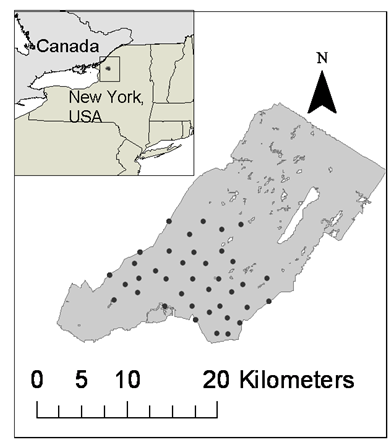
\includegraphics[height=2.5in,width=1.9in]{Ch3/figs/hairsnares.png}
\caption{Fort Drum study area and hair snare locations.}
\label{fig.3.bears1}
\end{figure}

{\small
\begin{verbatim}
# Consider adding comments to your code.
## Good idea. This will be done in final draft
trapmat<-read.csv("FDtrapmat.csv")
bearArray<-source("FDbeararray.R")$value
nind<-dim(bearArray)[1]
K<-dim(bearArray)[3]
ntraps<-dim(bearArray)[2]

M=175
nz<-M-nind

Xaug <- array(0, dim=c(M,ntraps,K))
Xaug[1:nind,,]<-bearArray
y<- apply(Xaug,c(1,3),sum)
y[y>1]<-1
ytot<-apply(y,1,sum)   # total encounters out of K
\end{verbatim}
}

Note that the raw data, ${\bf y}$, is an $M \times K$ array of
individual encounter events (i.e., $y_{ik} = 1$ if individual $i$ was
encountered in any trap and 0 otherwise).  For $i=48,...,175$,
$y_{ik}$=0 as these are augmented observations.  For Model M0 it is
sufficient to reduce the data to individual encounter frequencies
which we have labeled \mbox{\tt ytot} above.  The BUGS model file
along with commands to fit the model are as follows:

{\small
\begin{verbatim}
set.seed(2013)               # to obtain the same results each time
data0<-list(y=y,M=M,K=K)
params0<-list('psi','p','N')
zst=c(rep(1,nind),rbinom(M-nind, 1, .5))
inits =  function() {list(z=zst, psi=runif(1), p=runif(1)) }

cat("
model {

psi~dunif(0, 1)
p~dunif(0,1)

for (i in 1:M){
   z[i]~dbern(psi)
   for(k in 1:K){
      tmp[i,k]<-p*z[i]
      y[i,k]~dbin(tmp[i,k],1)
       }
       }
N<-sum(z[1:M])
}
",file="modelM0.txt")

fit0 = bugs(data0, inits, params0, model.file="modelM0.txt",
       n.chains=3, n.iter=2000, n.burnin=1000, n.thin=1,
       debug=TRUE,working.directory=getwd())
\end{verbatim}
}

The posterior
 summary statistics from this analysis are as follows:
{\small
\begin{verbatim}
> print(fit0,digits=2)
Inference for Bugs model at "modelM0.txt", fit using WinBUGS,
 3 chains, each with 2000 iterations (first 1000 discarded)
 n.sims = 3000 iterations saved
           mean    sd   2.5%    25%    50%    75%  97.5% Rhat n.eff
psi        0.29  0.04   0.22   0.26   0.29   0.31   0.36    1  3000
p          0.30  0.03   0.25   0.28   0.30   0.32   0.35    1  3000
N         49.94  1.99  47.00  48.00  50.00  51.00  54.00    1  3000
deviance 489.05 11.28 471.00 480.45 488.80 495.40 513.70    1  3000

[.. some output deleted ...]
\end{verbatim}
}
{\bf WinBUGS} did well in choosing an MCMC algorithm for this model --
we have $\hat{R} = 1$ for each parameter, and an effective sample size
of 3000, equal to the total number of posterior samples.
We see that the posterior mean of $N$ under this
model is $49.94$ and a 95\% posterior interval is $(48,54)$.  We
revisit these data later in the context of more complex models.



In order to obtain an estimate of density, $D$, we need an area to
associate with the estimate of $N$, and commonly used procedures to
conjure up such an area include buffering the trap array by the home
range radius, often estimated by the mean maximum distance moved
(MMDM)\footnote{really MMDM? How can this be an estimate of the home
  range radius? Reference for this?}, $1/2$ MMDM \citep{dice:1938} or
directly from telemetry data (REF XXX NEED REF HERE XXXXX). Typically, the trap
array is defined by the convex hull around the trap locations, and
this is what we applied a buffer to. We computed the buffer by using
an estimate of the mean female home range radius (2.19 km) estimated from
telemetry studies \citep{bales_etal:2005} instead of using an estimate
based on our relatively more sparse recapture data\footnote{BETH:
  Why?}.
 For the Fort Drum study, the convex hull has area
$157.135$ $km^2$, and the buffered convex hull has area $277.011$
$km^2$.
To create this we used functions contained in the {\bf R} package
\mbox{\tt rgeos} and created a utility function \mbox{\tt bcharea}
which is in our {\bf R} package \mbox{\tt scrbook}. The commands are
as follows:
\begin{verbatim}
library("rgeos")

bcharea<-function(buff,traplocs){
p1<-Polygon(rbind(traplocs,traplocs[1,]))
p2<-Polygons(list(p1=p1),ID=1)
p3<-SpatialPolygons(list(p2=p2))
p1ch<-gConvexHull(p3)
 bp1<-(gBuffer(p1ch, width=buff))
 plot(bp1, col='gray')
 plot(p1ch, border='black', lwd=2, add=TRUE)
 gArea(bp1)
}

bcharea(2.19,traplocs=trapmat)
\end{verbatim}
The resulting buffered convex hull is shown in Fig. \ref{closed.fig.bch}.
\begin{figure}
\begin{center}
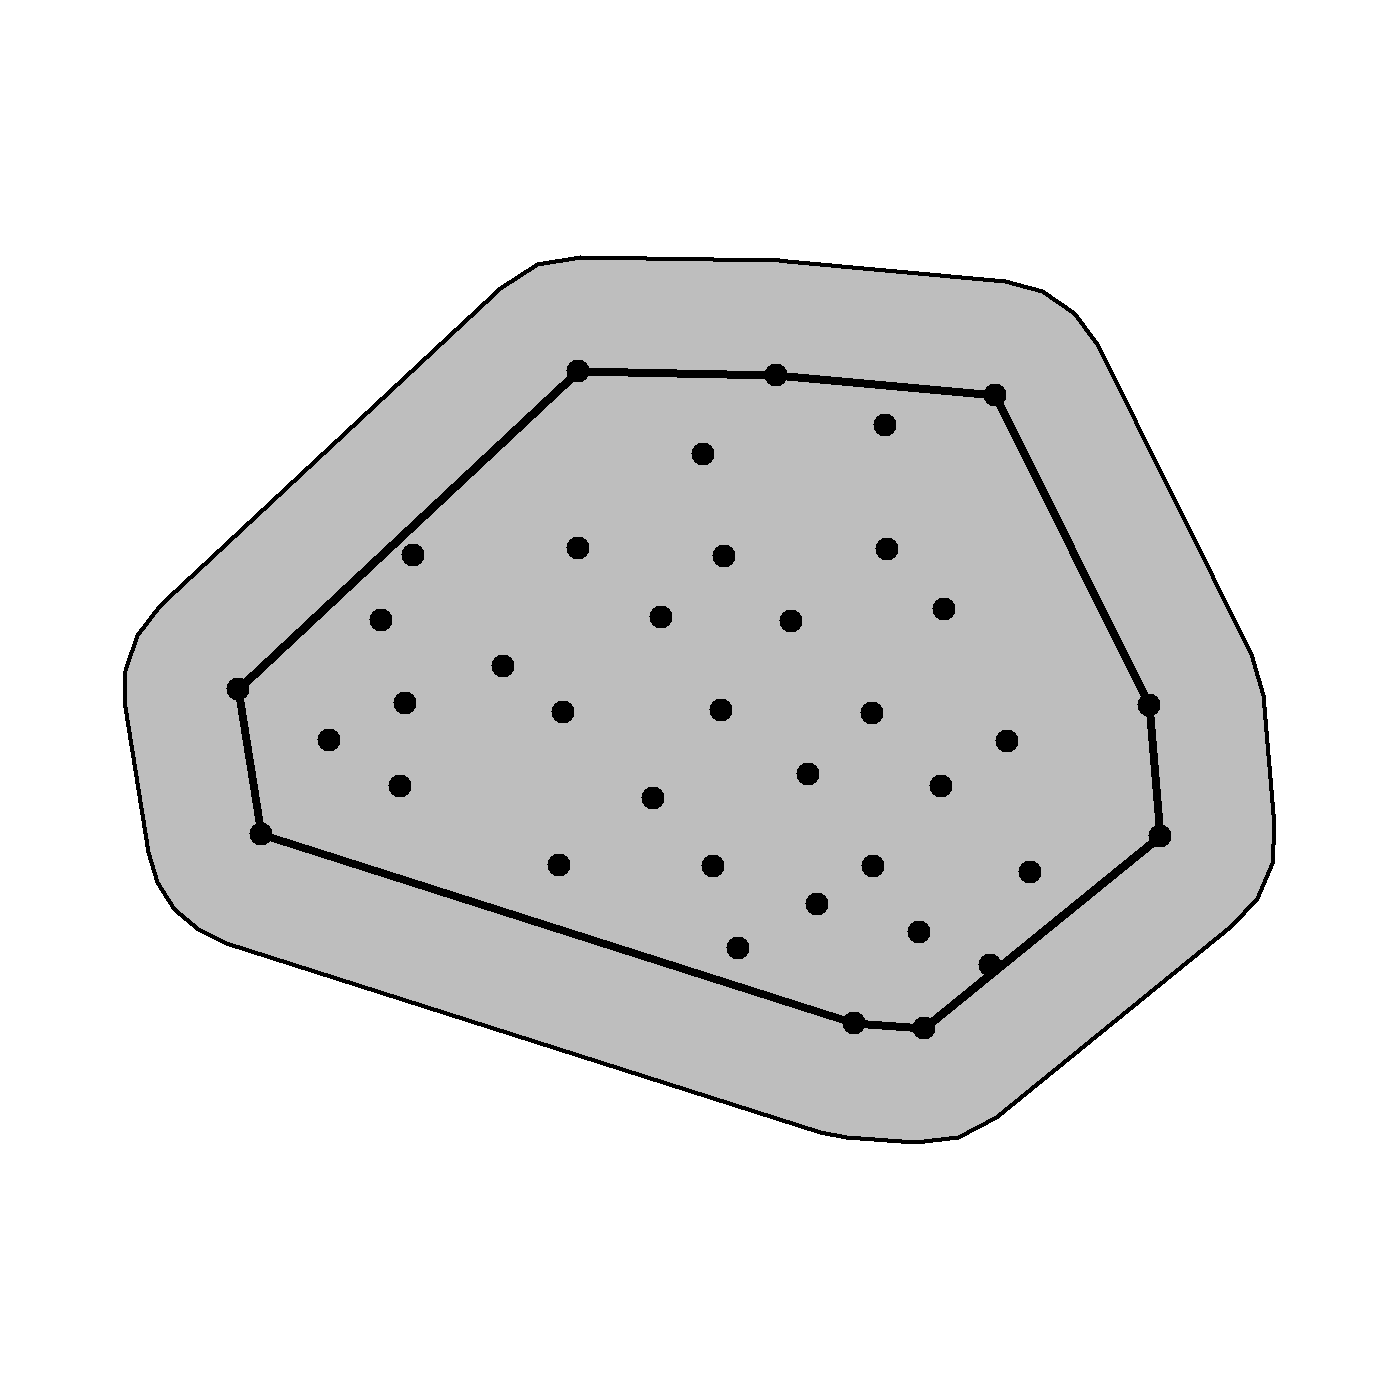
\includegraphics[height=3in,width=3in]{Ch3/figs/bufferedCH}
\end{center}
\caption{buffered convex hull of the bear hair snare array}
\label{closed.fig.bch}
\end{figure}

To conjure up a
density estimate under model $M_0$, we compute the appropriate
posterior summary of $N$ and the prescribed area ($277.011$ $km^2$):
\begin{verbatim}
> summary(fit0$sims.list$N/277.011)
   Min. 1st Qu.  Median    Mean 3rd Qu.    Max.
 0.1697  0.1733  0.1805  0.1803  0.1841  0.2130

> quantile(fit0$sims.list$N/277.011,c(0.025,0.975))
     2.5%     97.5%
0.1696684 0.1949381
\end{verbatim}
which yields a density estimate of about $0.18$ ind/km$^2$, and a $95\%$ Bayesian
confidence interval of $(0.170, 0.195)$.

The obvious limitation of this estimate and, indeed, of the whole
process, is that our choice of ``area'' is completely subjective -
which area should we use? MMDM? One-half MMDM? Estimated from
telemetry data? And, furthermore, how certain are we of this area? Can
we quantify our uncertainty about this quantity?
 More important, what exactly is
the meaning of this area and, in this context, how do we gauge bias
and/or variance of ``estimators'' of it? (i.e., what is it
estimating?).

\section{Temporally varying and behavioral effects}

The purpose of this chapter is mainly to emphasize the central
importance of the binomial model in capture-recapture and so we have
considered models for individual encounter frequencies - the number of
times individuals are captured out of $K$ samples.  Sometimes it is
not acceptable to aggregate the encounter data for each individual --
such as when encounter probability varies over time among samples. A
type of time-varying response that seems relevant in most
capture-recapture studies is ``effort'' such as amount of search time,
number of observers, or trap effort
 or when $p$ depends on date
\citep{kery_etal:2010, gardner_etal:2010}.
  A common situation is that in
which there exists a ``behavioral response'' to trapping (even if the
animal is not physically trapped).

Behavioral response is an important concept in carnivore studies
because individuals might learn to come to baited traps or avoid traps
due to trauma related to being encountered.  There are a number of
ways to parameterize a behavioral response to encounter. The
distinction between persistent and ephemeral was made by
\citet{yang_chao:2005} who considered a general behavioral response
model of the form:
\[
\mbox{logit}(p_{ik}) = \alpha_{0} + \alpha_{1}*y_{i,k-1} + \alpha_{2} x_{ik}
\]
where $x_{ik}$ is a covariate indicator variable of previous capture
(i.e., $x_{ik} = 1$ if captured in any previous period). Therefore,
encounter probability changes depending on whether an individual was
captured in the immediate previous period (ephemeral behavioral
response) or in any previous period (persistent behavioral
response). The former probably models a behavioral response due to
individuals moving around their territory relatively slowly over time
and the latter probably accommodates trap happiness due to baiting or
shyness due to trauma.  In spatial capture-recapture models it makes
sense to consider a local behavioral response that is trap-specific
\citep{royle_etal:2011jwm} - that is, the encounter probability is
modified for individual traps depending on previous capture in
specific traps.

Models with temporal effects are easy to describe in the {\bf BUGS} language
and analyze and we provide a number of examples in chapt. 8. XXXXX ?? XXXXX


\section{ Models with individual heterogeneity}
\label{closed.sec.modelmh}



Here we consider models with individual-specific encounter probability
parameters, say $p_{i}$, which we model according to some probability
distribution, $g(\theta)$. We denote this basic model assumption as
$p_{i} \sim g(\theta)$. This type of model is similar in concept to
extending a GLM to a GLMM but in the capture-recapture context $N$ is
unknown.  The basic class of models is often referred to as ``Model
$M_h$'' but really this is a broad class of models, each being
distinguished by the specific distribution assumed for $p_{i}$.  There
are many different varieties of Model $M_{h}$ including parametric and
various putatively non-parametric approaches
\citep{burnham_overton:1978, norris_pollock:1996, pledger:2000}. One
important practical matter is that estimates of $N$ can be extremely
sensitive to the choice of heterogeneity model
\citep{fienberg_etal:1999, dorazio_royle:2003, link:2003}. Indeed,
\citet{link:2003} showed that in some cases it's possible to find
models that yield precisely the same expected data, yet produce wildly
different estimates of $N$. In that sense, $N$ for most practical
purposes is not identifiable across classes of mixture models, and
this should be understood before fitting any such model. One solution
to this problem is to seek to model explicit factors that contribute
to heterogeneity, e.g., using individual covariate models (See
\ref{closed.sec.indcov} below). Indeed, spatial capture-recapture
models seek to do just that, by modeling heterogeneity due to the
spatial organization of individuals in relation to traps or other
encounter mechanism.  For additional background and applications of
Model $M_{h}$ see \citet[][chapt. 6]{royle_dorazio:2008} and
\citet[][chapt. 6]{kery_schaub:2011}.

Model $M_{h}$ has important historical relevance to spatial
capture-recapture situations \citep{karanth:1995} because
investigators recognized that the juxtaposition of individuals with
the array of trap locations should yield heterogeneity in encounter
probability, and thus it became common to use some version of Model $M_h$
in spatial trapping arrays to estimate $N$.  While this doesn't
resolve the problem of not knowing the area relevant to $N$, it does
yield an estimator that accommodates the heterogeneity in $p$ induced
by the spatial aspect of capture-recapture studies.

To see how this juxtaposition induces heterogeneity, we have to
understand the relevance of movement in capture-recapture models.
Imagine a quadrat that can be uniformly searched by a crew of
biologists for some species of reptile (see
\citet{royle_young:2008}).  Figure \ref{closed.fig.quadrat} shows a
sample quadrat searched repeatedly over a period of time. Further,
suppose that species exhibits some sense of spatial fidelity in the
form of a home range or territory, and individuals move about their
home range (home range centroids are given by the blue dots) in some
kind of random fashion.  It is natural to think about it in terms of a
movement process and sometimes that movement process can be modeled
explicitly using hierarchical models \citep{royle_young:2008,
  royle_etal:2011mee}.  Heuristically, we imagine that each individual in
the vicinity of the study area is liable to experience variable
exposure to encounter due to the overlap of its home range with the
sampled area - essentially the long-run proportion of times the
individual is within the sample plot boundaries, say $\phi$. We
might model the exposure of an individual to capture by supposing that
$z_{i} = 1$ if individual $i$ is available to be captured (i.e.,
within the survey plot) during any sample, and $0$ otherwise. Then,
$\Pr(z_{i}=1) = \phi$.  In the context of spatial studies, it is
natural that $\phi$ should depend on {\it where} an individual lives,
i.e., it should be individual-specific $\phi_{i}$
\citep{chandler_etal:2011}. This system describes, precisely, that of
``random temporary emigration'' \citep{kendall_etal:1997} where $\phi_{i}$
is the individual-specific probability of being ``available'' for
capture.

Conceptually, SCR models aim to deal with
this problem of variable exposure to sampling due to movement in the
proximity of the trapping array explicitly and formally with auxiliary
spatial information.  If individuals are detected with probability
$p_{0}$, {\it conditional} on $z_{i} = 1$, then the marginal
probability of detection of individual $i$ is
\[
 p_{i} = p_{0}\phi_{i}
\]
so we see clearly that individual heterogeneity in encounter
probability is induced as a result of the juxtaposition of individuals
(i.e., their home ranges) with the sample apparatus and the movement
of individuals about their home range.

\begin{figure}
\begin{center}
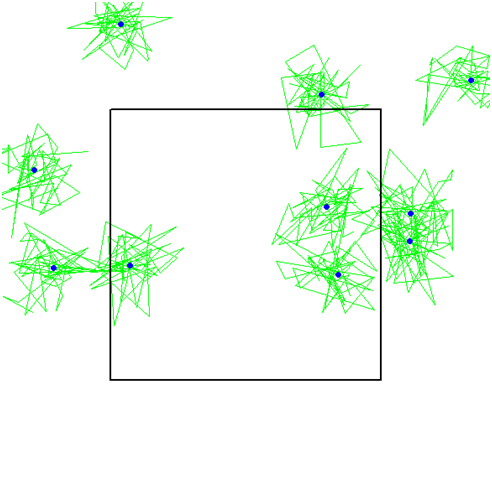
\includegraphics[height=3in]{Ch3/figs/quadrat}
\end{center}
\caption{A quadrat searched for lizards and the locations of each
  lizard over some period of time.}
\label{closed.fig.quadrat}
\end{figure}

We will work with a specific type of Model $M_{h}$ here, that in which
we extend the basic binomial observation model of Model $M_{0}$ so
that
\[
\mbox{logit}(p_{i}) = \mu + \eta_{i}
\]
where
\[
\eta_{i} \sim \mbox{Normal}(0, \sigma_{p}^2)
\]
We could as well write
\[
\mbox{logit}(p_{i}) \sim \mbox{Normal}(\mu,\sigma_{p}^2)
\]
This ``logit-normal mixture'' was analyzed by
\citet{coull_agresti:1999} and elsewhere. It is a natural extension of
the basic model with constant $p$, as a mixed GLMM, and similar models
occur throughout statistics. It is also natural to consider a beta
prior distribution for $p_{i}$ \citep{dorazio_royle:2003} and
so-called ``finite-mixture'' models are also popular
\citep{norris_pollock:1996, pledger:2000}.

\subsection{Analysis of Model Mh}

If $N$ is known, it is worth taking note of the essential simplicity
of Model $M_h$ as a binomial GLMM.  This is a type of model that is
widely applied in just about every scientific discipline and using
standard methods of inference based either on integrated likelihood
\citep{laird_ware:1982, berger_etal:1999} which we discuss in
chapt. \ref{chapt.mle} or standard Bayesian
methods. However, because $N$ is not known, inference is somewhat more
challenging. We address that here using Bayesian analysis based on
data augmentation (DA). Although we use data augmentation in the context of
Bayesian methods here, we note that
heterogeneity models formulated under DA are easily analyzed by
conventional likelihood methods as zero-inflated binomial mixtures
\citep{royle:2006} and more traditional analysis of model $M_h$ based on
integrated likelihood, without using data augmentation, has been
considered by \citet{coull_agresti:1999}, \citet{dorazio_royle:2003},
and others.

As with model $M_{0}$, we have the Bernoulli model for the
zero-inflation variables: $z_{i} \sim \mbox{Bern}(\psi)$ and the model
of the observations expressed conditional on the latent variables
$z_{i}$. For $z_{i}=1$, we have a binomial model with
individual-specific $p_{i}$:
\[
y_{i}|{z_{i} \! = \! 1} \sim \mbox{Bin}(K,p_{i})
\]
and otherwise $y_{i} |{ z_{i} \! = \! 0} \sim \delta(0)$. Further, we
prescribe a distribution for $p_{i}$. Here we assume
\[
\mathrm{logit}(p_{i}) \sim \mbox{Normal}(\mu,\sigma^2)
\]
The basic {\bf BUGS} description for this model, assuming a
$\mbox{Unif}(0,1)$ prior for $p_{0} = \mbox{logit}^{-1}(\mu)$, is given
as follows:
{\small
\begin{verbatim}
model{

p0 ~ dunif(0,1)       # prior distributions
mup<- log(p0/(1-p0))
taup~dgamma(.1,.1)
psi~dunif(0,1)

for(i in 1:(nind+nz)){
  z[i]~dbern(psi)     # zero inflation variables
  lp[i] ~ dnorm(mup,taup) # individual effect
  logit(p[i])<-lp[i]
  mu[i]<-z[i]*p[i]
  y[i]~dbin(mu[i],J)  #  observation model
 }

N<-sum(z[1:(nind+nz)])  # N is a derived parameter
}
\end{verbatim}
}


\subsection{Analysis of the Fort Drum data}

The logit-normal heterogeneity model was fitted to the bear data from
the Fort Drum study, and we used data augmentation to produce a data
set of $M=500$ individuals.  We ran the model using {\bf JAGS} with
the instructions given as follows\footnote{For WinBUGS, should provide
  starts for lp and sigma or sometimes WinBUGS breaks}.
{\small
\begin{verbatim}
[... get data as before ....]

set.seed(2013)

cat("
model{
p0 ~ dunif(0,1)       # prior distributions
mup<- log(p0/(1-p0))
sigmap ~ dunif(0,10)
taup<- 1/(sigmap*sigmap)
psi~dunif(0,1)

for(i in 1:(nind+nz)){
  z[i]~dbern(psi)     # zero inflation variables
  lp[i] ~ dnorm(mup,taup) # individual effect
  logit(p[i])<-lp[i]
  mu[i]<-z[i]*p[i]
  y[i]~dbin(mu[i],K)  #  observation model
 }

N<-sum(z[1:(nind+nz)])
}
",file="modelMh.txt")

data1<-list(y=ytot, nz=nz, nind=nind,K=K) 
params1= c('p0','sigmap','psi','N')
inits =  function() {list(z=as.numeric(ytot>=1), psi=.6, p0=runif(1),
          sigmap=runif(1,.7,1.2),lp=rnorm(M,-2)) }

library("rjags")
jm<- jags.model("modelMh.txt", data=data1, inits=inits, n.chains=4,
                 n.adapt=1000)
jout<- coda.samples(jm, params1, n.iter=200000, thin=1)
\end{verbatim}
}
This produces the posterior distribution for $N$ shown
in Fig. \ref{closed.fig.bearMh}. Posterior summaries of parameters are
given as follows:
{\small
\begin{verbatim}
> summary(jout)

Iterations = 2001:202000
Thinning interval = 1 
Number of chains = 4 
Sample size per chain = 2e+05 

1. Empirical mean and standard deviation for each variable,
   plus standard error of the mean:

           Mean       SD  Naive SE Time-series SE
N      117.7740 56.31633 6.296e-02       1.960115
p0       0.0728  0.05522 6.174e-05       0.001655
psi      0.2366  0.11362 1.270e-04       0.003909
sigmap   2.0795  0.53096 5.936e-04       0.016789

2. Quantiles for each variable:

            2.5%      25%       50%      75%    97.5%
N      62.000000 82.00000 102.00000 134.0000 277.0000
p0      0.003143  0.02842   0.06077   0.1066   0.2036
psi     0.117269  0.16377   0.20522   0.2712   0.5560
sigmap  1.211900  1.69434   2.02113   2.4028   3.2694
\end{verbatim}
}


We used $M=500$ for this analysis and we
note that  while the posterior mass of $N$ is concentrated away from this
upper bound (Fig. \ref{closed.fig.bearMh}), the posterior has an
extremely long right tail, with some posterior values at the upper
bound $N=500$. Maybe or
maybe not sufficient data augmentation.\footnote{
{\bf to do: } insert final results. longer run. more data
augmentation. compare with winbugs.
}
The model runs effectively in {\bf WinBUGS} but sometimes with apparently
inefficient mixing for reasons that may be related to bad starting
values. In some cases this was resolved if we supplied starting values
for the $logit(p_{i})$ parameters and $\tau$.


Because of the skewed posterior we see that the posterior mean ($N=117$)
is
considerably higher than the posterior mode ($N=102$). Moreover, 
posterior summaries are estimated with a relatively high error
(``Time-series SE'' of around 2.0)\footnote{need to define this somewhere}.
Further, it may be surprising that the posterior mode does not compare
well with the MLE. To compute the posterior mode we could easily find
the posterior value of $N$ with the highest mass because $N$ is
discrete. But we want to smooth out some of the Monte Carlo error a
bit so we used a smoothing spline to the posterior frequencies of $N$
as follows:
\begin{verbatim}
>  tt<-table(jout[[1]][,"N"])[1:80]
>  xg<-as.numeric(names(tt))
>  plot(xg,tt)
>  sp<- smooth.spline(xg,tt,df=9)
>  sp$x[sp$y==max(sp$y)]
[1] 80
\end{verbatim}
The \mbox{\tt df} argument controls the degree of smoothing and we
find in this case that the modal value (i.e., 80) is not too sensitive
to the smoothing parameter but this should be checked in any specific
instance\footnote{we need to give examples of using \mbox{\tt
    density()} to obtain modes}.

To compare with the MLE, we used 
the {\bf R} code contained in Panel 6.1 of \citet{royle_dorazio:2008}.  The
MLE of $log(n_{0})$, the logarithm of the number of uncaptured
individuals, is $log(n0) = 3.86$ and therefore the MLE is $\hat{N} =
exp(3.86)+47 = 94.47$ which is not at all consistent with the apparent
mode in 
Fig. \ref{closed.fig.bearMh}.
\footnote{We note that the result is inconsistent with Gardner et
  al. (2009) who reported an MLE of 104.1 ($density = 0.437
  inds/km^2$) although we do not know the reason for this at the
  present time.}  
%To convert this to density we use the buffered area
%as computed above (255.3 $km^2$)\footnote{WRONG \#} and perform the
%required summary analysis on the posterior samples of $N$, which
%results in about $0.37$ individuals/$km^2$. The reader should carry
%out this analysis to confirm the estimates, and also obtain the $95\%$
%confidence interval.

Comments: First of all the posterior for this model and data set is
very sensitive to prior distributions. While MLEs are invariant to
transformation of the parameters, the posterior distribution
definitely is {\it not} invariant. In the present case, the use of a
$\mbox{Unif}(0,1)$ prior for $p_{0} = expit(\mu)$ is somewhat
informative -- in particular, it is not at all ``flat'' on the scale
of $\mu$ -- and this affects the posterior.  We generally always
recommend use of a $Unif(0,1)$ prior for $expit(\mu)$ in such
models. That said, we were surprised at this result, and we
experimented with other prior configurations including putting a flat
prior on $\mu$ directly. This specific prior suggests the possibility
that the posterior distribution may be improper for that prior
specification. This kind of small sample instability has been widely
noted in Model Mh \citep{fienberg_etal:1999, dorazio_royle:2003} and
is not unrelated to sensitivity to
model which has also been identified as an important issue in model
$M_{h}$ \citep{dorazio_royle:2003,link:2003}.
Conclusion: The mode is well-defined but the data set is sparse and
hence inferences are poor and sensitive to model choices. Get over it.


\begin{figure}
\centering
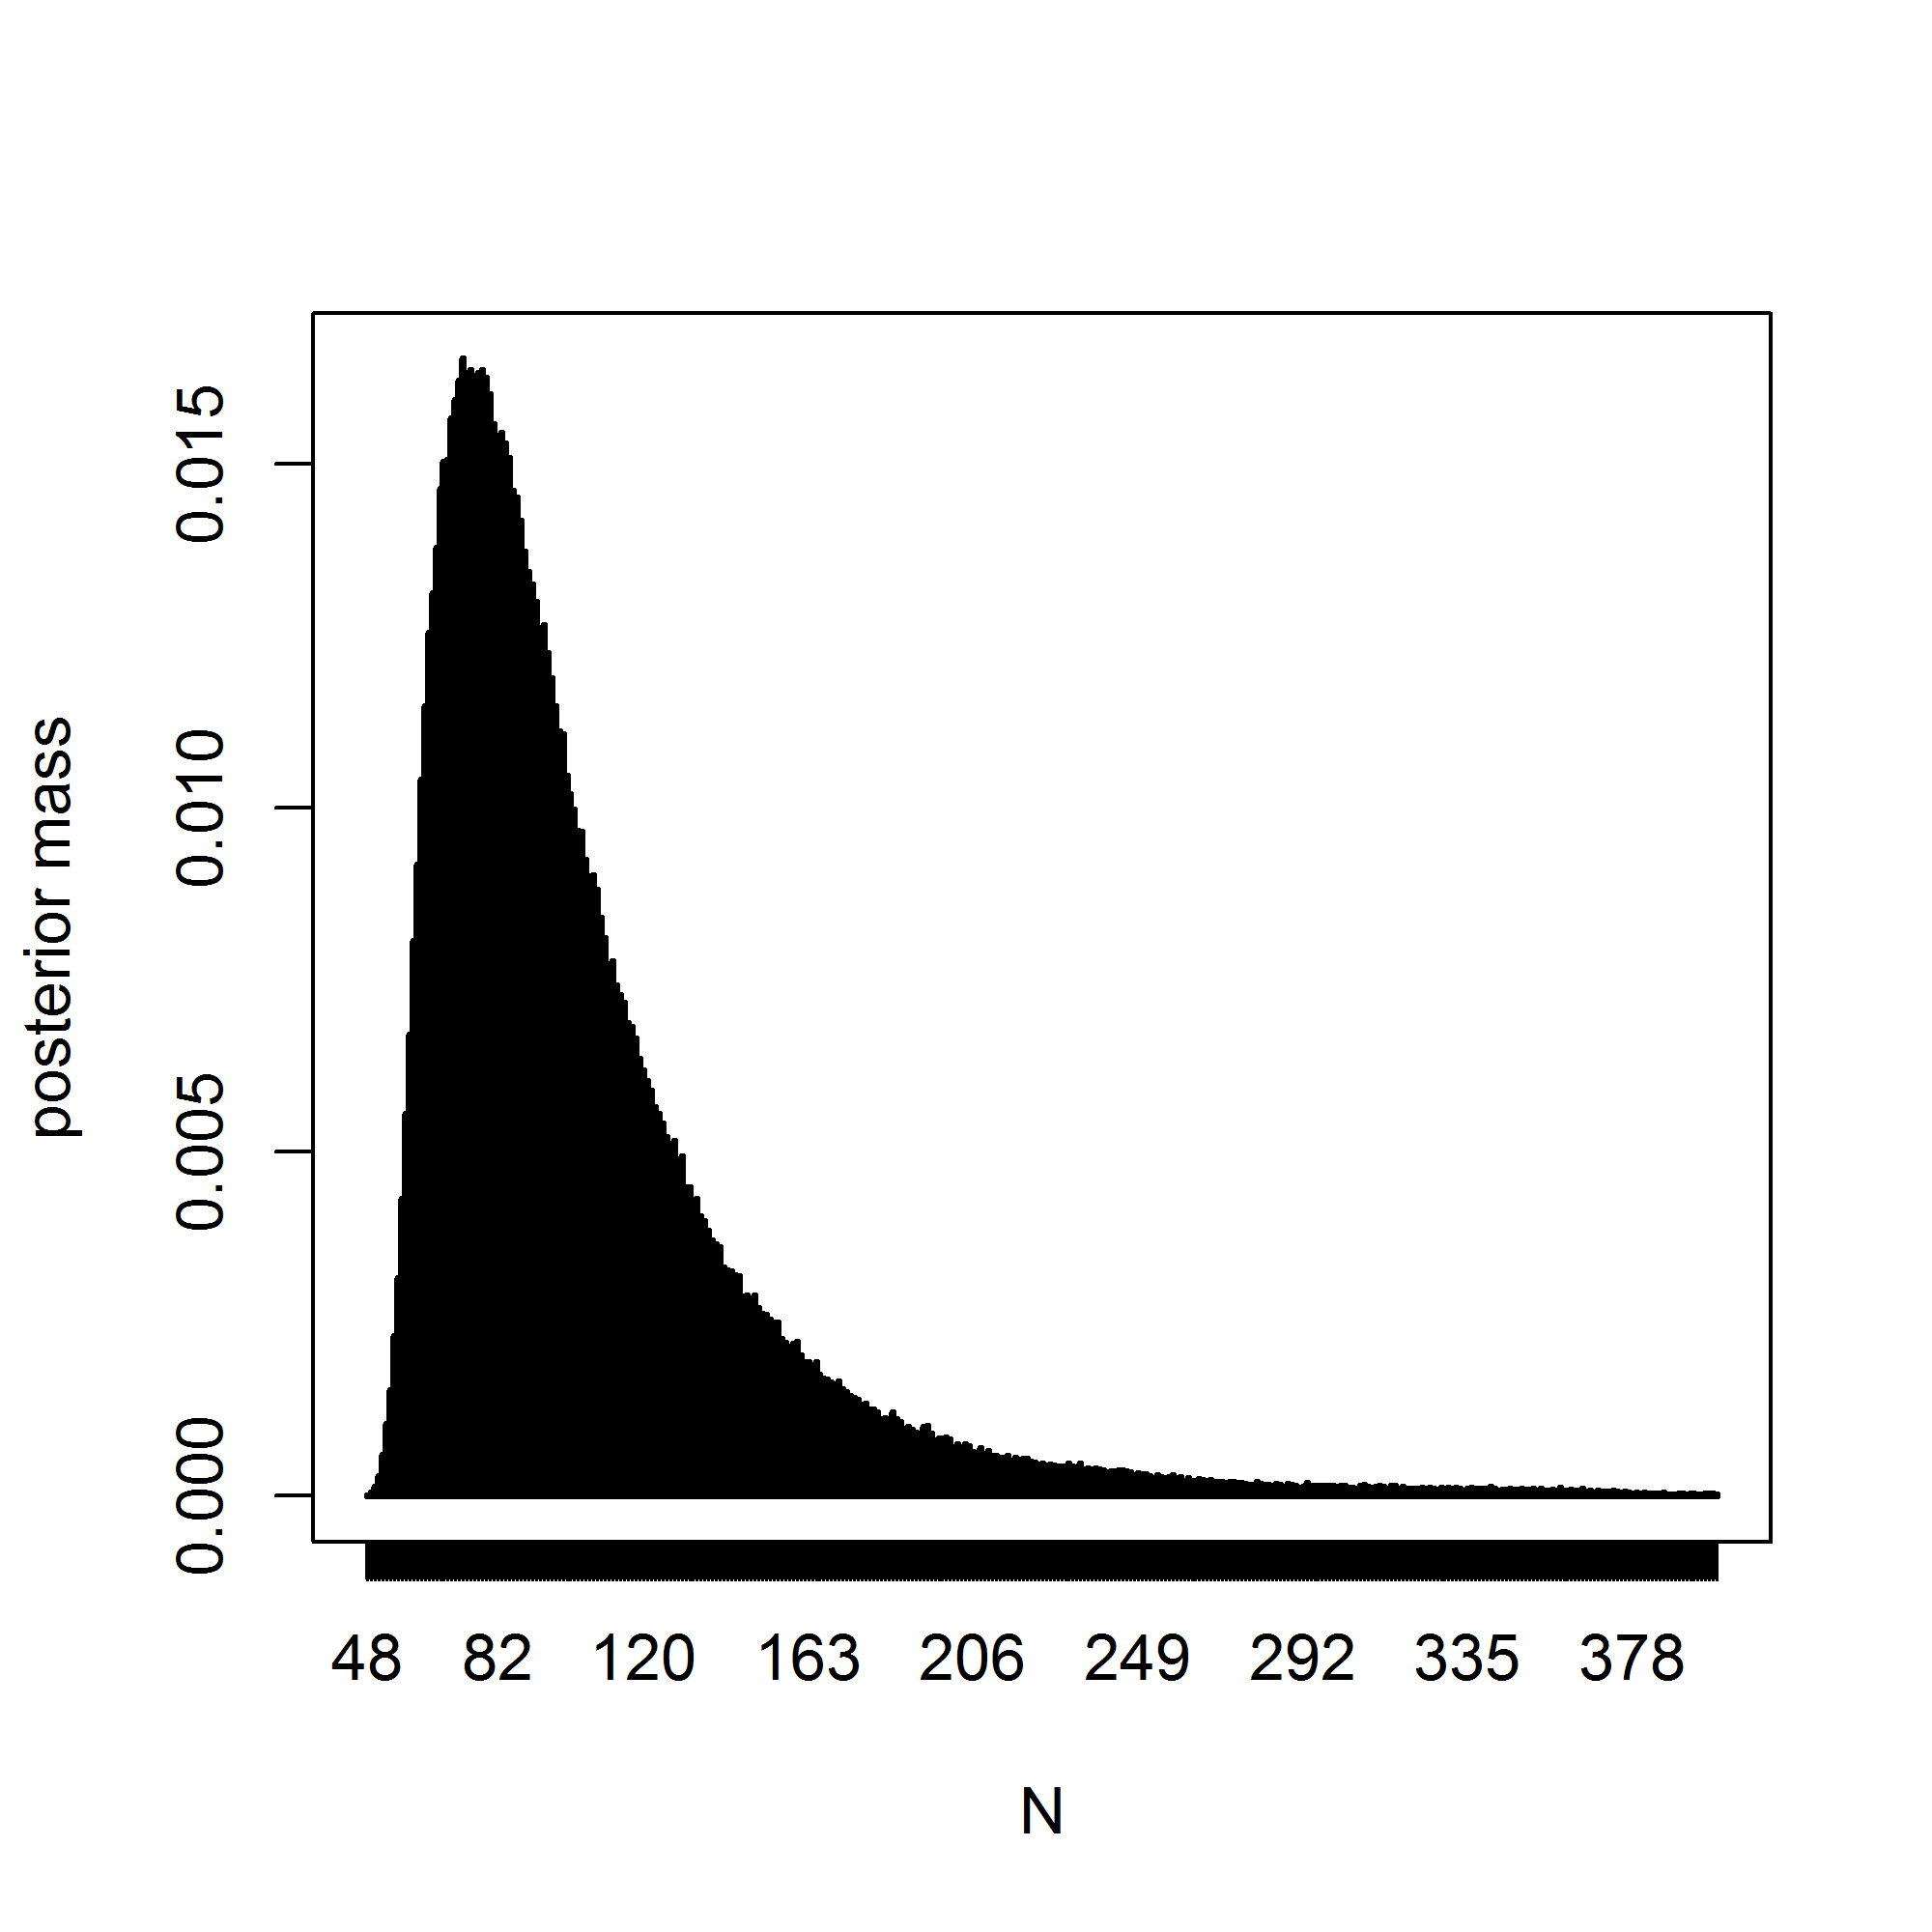
\includegraphics[height=4.5in,width=4.5in]{Ch3/figs/bear-modelMh-post}
\caption{Posterior of $N$ for Fort Drum bear study data under the
logit-normal version of model $M_h$. From WinBUGS output. 200k
samples.
}
\label{closed.fig.bearMh}
\end{figure}


\subsection{Building your own MCMC algorithm}

For fun, we construct our own MCMC algorithm using a Metropolized
Gibbs sampler for Model $M_{h}$.  In chapter \ref{chapt.mcmc} we devise MCMC
algorithms for spatial capture-recapture models and the basic
conceptual and technical considerations are entirely analogous to
Model $M_h$.

To begin, we first collect all of our model components
which are as follows: $[y_{i}| p_{i},z_{i}]$,
$[p_{i}|\mu_{p},\sigma_{p}]$, and $[z_{i}|\psi]$
for {\it each} $i=1,2,\ldots,M$ and then prior distributions
$[\mu_{p}]$, $[\sigma_{p}]$ and $[\psi]$.
The joint posterior distribution of all unknown quantities in the model
is proportional to the joint distribution of all elements
$y_{i},p_{i},z_{i}$ and also the prior distributions of the prior parameters:
\[
\left\{ \prod_{i=1}^{M} [y_{i}|p_{i},z_{i}][p_{i}|\mu_{p},\sigma_{p}]
[z_{i}|\psi] \right\} [\mu_{p},\sigma_{p},\psi]
\]
For prior distributions, we assume that $\mu_{p},\sigma_{p}, \psi$ are
mutually independent and for $\mu_{p}$ and $\sigma_{p}$ we use
improper uniform priors, and $\psi \sim \mbox{Unif}(0,1)$.  Note that
the likelihood contribution for each individual, when conditioned on
$p_{i}$ and $z_{i}$, does not depend on $\psi$, $\mu_{p}$, or
$\sigma_{p}$.  As such, the full-conditionals for the structural
parameters $\psi$ only depends on the collection of data augmentation
variables $z_{i}$, and that for $\mu_{p}$ and $\sigma_{p}$ will only
depends on the collection of latent variables $p_{i}; i=1,2,\ldots,M$.
The full conditionals for all the unknowns are as follows:

{\bf (1)} For $p_{i}$:
\begin{eqnarray*}
[p_{i}|y_{i}, \mu_p, \sigma_{p},z_{i}=1] &\propto  &
[y_{i}|p_{i}][p_{i}|\mu_p,\sigma_{p}^{2}] \mbox{ if $z_{i}=1$ }  \\
                 &  &  [p_{i}|\mu_p,\sigma_{p}] \mbox{if $z_{i}=0$ }
\end{eqnarray*}

{\bf (2)} for $z_{i}$:
\[
z_{i} | \cdot \propto [y_{i}|z_{i}*p_{i}] \mbox{Bern}(z_{i}|\psi)
\]

{\bf (3)} For $\mu_{p}$:
\[
[\mu_{p} | \cdot ] \sim \prod_{i} [p_{i}| \cdot] *\mbox{const}
\]


{\bf (4)} For $\sigma_{p}$:
\[
[ \sigma_{p}|\cdot ] \sim\prod_{i}[p_{i}| \cdot ]*\mbox{const}
\]

{\bf (5)} For $\psi$:
\[
\psi|\cdot\sim \mbox{Beta}(1 + \sum z_{i}, 1 + M - \sum z_{i})
\]


We've  identified each of the full conditional
distributions in sufficient detail to apply the
Metropolis-Hastings algorithm. With the exception of $\psi$ which has
a convenient analytic solution -- it is a beta distribution which we
can easily sample directly. In truth, we could also sample $\mu_{p}$
and $\sigma_{p}^{2}$ directly with certain choices of prior
distributions. For example, if $\mu_{p} \sim \mbox{Normal}(0, 1000)$
then the full conditional for $\mu_{p}$ is also normal, etc..
We implement an MCMC algorithm for this model in the following block
of {\bf R} code.  The basic structure is: initialize the parameters
and create any required output or intermediate data holders, and then
begin the main MCMC loop which, in this case, generates 100000
samples.\footnote{This data grabbing function is not implemented yet}

{\small
\begin{verbatim}
## obtain the bear data by executing the previous data grabbing
## function

temp<-getdata()
M<-temp$M
K<-temp$K
ytot<-temp$ytot

###
### MCMC algorithm for Model Mh

out<-matrix(NA,nrow=100000,ncol=4)
dimnames(out)<-list(NULL,c("mu","sigma","psi","N"))
lp<- rnorm(M,-1,1)
p<-expit(lp)
mu<- -1
p0<-exp(mu)/(1+exp(mu))
sigma<- 1
psi<- .5
z<-rbinom(M,1,psi)
z[ytot>0]<-1

for(i in 1:100000){

### update the logit(p) parameters
lpc<- rnorm(M,lp,1)  # 0.5 is a tuning parameter
pc<-expit(lpc)
lik.curr<-log(dbinom(ytot,K,z*p)*dnorm(lp,mu,sigma))
lik.cand<-log(dbinom(ytot,K,z*pc)*dnorm(lpc,mu,sigma))
kp<- runif(M) < exp(lik.cand-lik.curr)
p[kp]<-pc[kp]
lp[kp]<-lpc[kp]

p0c<- rnorm(1,p0,.05)
if(p0c>0 & p0c<1){
muc<-log(p0c/(1-p0c))
lik.curr<-sum(dnorm(lp,mu,sigma,log=TRUE))
lik.cand<-sum(dnorm(lp,muc,sigma,log=TRUE))
if(runif(1)<exp(lik.cand-lik.curr)) {
 mu<-muc
 p0<-p0c
}
}

sigmac<-rnorm(1,sigma,.5)
if(sigmac>0){
lik.curr<-sum(dnorm(lp,mu,sigma,log=TRUE))
lik.cand<-sum(dnorm(lp,mu,sigmac,log=TRUE))
if(runif(1)<exp(lik.cand-lik.curr))
 sigma<-sigmac
}

### update the z[i] variables
zc<-  ifelse(z==1,0,1)  # candidate is 0 if current = 1, etc..
lik.curr<- dbinom(ytot,K,z*p)*dbinom(z,1,psi)
lik.cand<- dbinom(ytot,K,zc*p)*dbinom(zc,1,psi)
kp<- runif(M) <  (lik.cand/lik.curr)
z[kp]<- zc[kp]

psi<-rbeta(1, sum(z) + 1, M-sum(z) + 1)

out[i,]<- c(mu,sigma,psi,sum(z))
}
\end{verbatim}
}


{\bf Remarks}: (1) for parameters with bounded support, i.e.,
$\sigma_{p}$ and $p_{0}$, we are using a random walk candidate
generator but rejecting draws outside of the parameter space.  (2) We
mostly use Metropolis-Hastings except for the data augmentation
parameter $\psi$ which we sample directly from its full-conditional
distribution which is a beta distribution.  (3) Even the latent data
augmentation variables $z_{i}$ are updated using Metropolis-Hastings
although they too can be updated directly from their full-conditional.

\subsection{Exercises related to model Mh}

\begin{itemize}
\item[(1)] Enclose the MCMC algorithm in an R function and provide
  arguments for some of the parameters of the function that a user
  might wish to modify.
\item[(2)] Execute the function and compare the results to those
  generated from WinBUGS in the previous section
\item[(3)] Note that the prior distribution for the ``mean'' parameter
  is given on $p_0=exp(\mu)/(1+exp(\mu))$.  Reformulate the algorithm
  with a flat prior on $\mu$ and see what happens. Contemplate this.
\item[(4)] Using Bayes rule, figure out the full conditional for
  $z_{i}$ so that you don't have to use MH for that one. It might be
  more efficient. Is it?
\item[(5)] Modify the MCMC algorithm so that the prior for $\mu_{p}$
  is an improper flat prior. i.e., $[\mu_{p}] \propto 1$. Describe the
  posterior distribution of $N$. 
\end{itemize}


\section{Individual Covariate Models: Toward Spatial Capture-Recapture}
\label{closed.sec.indcov}

{\bf ANDY STOPPED EDITING HERE}

A standard situation in capture-recapture models is when an individual
covariate is measured, and this covariate is thought to influence
encounter probability.  As with other closed population models, we
begin with the basic binomial observation model:
\[
y_{i} \sim \mbox{Bin}(K, p_{i})
\]
and we assume also  a model for encounter probability according to:
\begin{equation}
 \mbox{logit}(p_{i}) = \alpha + \beta x_{i}
\label{closed.eq.ha}
\end{equation}
Classical examples of covariates influencing detection probability are
type of animal (juvenile/adult or male/female), a continuous covariate
such as body mass \citep[][ch. 6]{royle_dorazio:2008}, or a
discrete covariate such as group or cluster size. For example, in
models of aerial survey data, it is natural to model detection
probabilities as a function of the observation-level individual
covariate, ``group size'' \citep{royle:2008, royle:2009,
  langtimm_etal:2011}.

Such ``individual covariate models'' are similar in structure to Model
$M_{h}$, except that the individual effects are {\it observed} for the
$n$ individuals that appear in the sample. These models are important
here because spatial capture-recapture models are precisely a form of
individual covariate model, an idea that we will develop here and
elsewhere. Specifically, they are such models, but where the
individual covariate is a partially observed latent variable similar..
That is, unlike Model Mh, we do have some direct information about the
latent variable, which comes from the spatial locations/distribution
of individual recaptures.

Traditionally, estimation of $N$ in individual covariate models is
achieved using methods based on ideas of unequal probability sampling
(i.e., Horwitz-Thompson estimation; see \citet{huggins:1989} and
\citet{alho:1990}). An estimator of $N$ is
\[
\hat{N} = \sum_{i}^{n} \frac{1}{\tilde{p}_{i}}
\]
where $\tilde{p}_{i}$ is the probability that individual $i$ appeared
in the sample.  That is, $\tilde{p}_{i} = \Pr(y_{i}>0)$
where, in closed population capture-recapture models, 
\[
\Pr(y_{i}>0) = (1- (1-p_{i})^K)
\]
where $p_{i}$ is a function of parameters $\alpha$ and $\beta$
according to
Eq. \ref{closed.eq.ha}.
In practice, parameters are estimated 
from the conditional-likelihood of the observed encounter histories
which is, for observation $y_{i}$, 
\[
{\cal L}(\alpha, \beta | y_{i}) = \frac{ \mbox{Bin}(y_{i}|\alpha,\beta) } { \tilde{p}_{i}}.
\]

Here we take a formal model-based approach to Bayesian analysis of
such models using data augmentation \citep{royle:2009}. Classical
likelihood analysis of the so-called ``full likelihood'' is covered 
 by \citet{borchers_etal:2002}.  For Bayesian analysis of
individual covariate models, because the individual covariate is
unobserved for the $N-n$ uncaptured individuals, we require a model to
describe variation among individuals, essentially allowing the sample
to be extrapolated to the population\footnote{weak argument}.  For our present purposes, we
consider a continuous covariate and we assume that it has a normal
distribution:
\[
x_{i} \sim \mbox{Normal}(\mu,\sigma^{2})
\]

Data augmentation can be applied directly to this class of models. In
particular, reformulation of the model under DA yields a basic
zero-inflated binomial model of the form:
\begin{eqnarray*}
z_{i} &\sim& \mbox{Bern}(\psi) \\
y_{i}|{z_{i}\! =\! 1} &\sim& \mbox{Bin}(K,p_{i}(x_{i})) \\
y_{i} |{ z_{i}\! =\! 0} &\sim& \delta(0)  \\
x_{i} & \sim & \mbox{Normal}(\mu,\sigma^{2})
\end{eqnarray*}
Fully spatial capture-recapture models use this
formulation with a latent covariate that is directly related to the
individual detection probability (see next Section). As with the
previous models, implementation is trivial in the {\bf BUGS} language. The
{\bf BUGS} specification is very similar to that for model $M_h$, but we
require the distribution of the covariate to be specified, along with
priors for the parameters of that distribution.


\subsection{Example: Location of capture as a covariate.}

If we had a regular grid of traps over some closed geographic system
then we imagine that the average location of capture would be a decent
estimate (heuristically) of an individual's home range center.
Intuitively some measure of typical distance from home range center to
traps for an individual should be a decent covariate to explain
heterogeneity in encounter probability, i.e., individuals with more
exposure to traps should have higher encounter probabilities and vice
versa.  A version of this idea was put forth by
\citet{boulanger_mclellan:2001} (see also \citet{ivan:2012}), but
using the Huggins-Alho estimator and with covariate ``distance to
edge'' of the trapping array. A limitation of this  approach is
that it does not provide a solution to the problem that the trap area
is fundamentally ill-defined, nor does it readily accommodate the
inherent and heterogeneous variation in this measured covariate.
But here we do this analysis anyway.................
Here, we provide an example of this type of heuristically motivated
approach using the fully model-based individual covariate model
described above analyzed by data augmentation. We take a slightly
different approach than that adopted by
\citet{boulanger_mclellan:2001}. By analyzing the full likelihood and
placing a prior distribution on the individual covariate, we resolve
the problem of having an ill-defined area over which the population
size is distributed. After you read later chapters of this book, it
will be apparent that SCR models represent a formalization of this
heuristic procedure.

For our purposes here, we define $x_{i} = ||{\bf s}_{i} - {\bf
  x}_{0}||$ where ${\bf s}_{i}$
is the average encounter location of individual $i$ and ${\bf x}_{0}$ is the
centroid of the trap array.  Conceptually, individuals in the middle
of the array should have higher probability of encounter and, as
$x_{i}$ increases, $p_{i}$ should therefore decrease. We note that we
have defined $s_{i}$ in terms of a sample quantity - the observed mean
- which is ad hoc but maybe satisfactory under the circumstances. That
said, for
an expansive, dense trapping grid then we might expect the sample mean
encounter location to be a good estimate of home range center but,
clearly this is biased for individuals that live around the edge (or
off) the trapping array. Regardless, it should be good enough for our
present purposes of demonstrating this heuristically appealing
application of an individual covariate model. A key point is that
$s_{i}$ is missing for each individual that is not encountered and
thus so is $x_{i}$. Thus,
it is a latent variable, or random effect, and we need therefore to
specify a probability distribution for it.
As a measurement of distance we know it must be
positive-valued. Also beyond a certain distance individuals should not
be exposed at all so we should be able to pick some large number
$D_{max}$ beyond which we ................ complete this though....
As such, we use this distribution for the individual covariate
``distance from center of the trap array''
\[
 x_{i} \sim uniform(0,D_{max})
\]
where $D_{max}$ is a specified constant.  In practice, people have
used distance from edge of the trap array but that is less easy to
define and compute.


\subsubsection{Fort Drum Bear Study}

We have to do a little bit of data processing to fit this individual
covariate model to the Fort Drum data. 
We compute the individual covariate ${\bf x}_{i}$ using the {\bf R} script
provided in \mbox{\tt scrbook}......


To define the maximum distance (maxD) from the centroid, we use that
of the farthest trap, and so maxD is computed as follows:

\begin{verbatim}
minx<- min(trapmat[,1]-Cx)
maxx<-max(trapmat[,1]-Cx)
miny<- min(trapmat[,2]-Cy)
maxy<- max(trapmat[,2]-Cy)
# most extreme point determines maxD
ul<- c(minx,maxy)
maxD<- sqrt(  (ul[1]-0)^2 + (ul[2]-0)^2)
\end{verbatim}

For the bear data the maxD was about 11.5 km. As such, the model
described above will produce an estimate of the population size of
bears within 11.5 units of the trap centroid\footnote{To be convincing
  this might  need a little bit of hand-holding}. The BUGS model
specification and R commands to package the data and fit the model are
as follows:

\begin{verbatim}
cat("
model{
p0 ~ dunif(0,1)       # prior distributions
mup<- log(p0/(1-p0))
psi~dunif(0,1)
beta~dnorm(0,.01)

for(i in 1:(nind+nz)){
  xcent[i]~dunif(0,maxD)
  z[i]~dbern(psi)     # DA variables
  lp[i] <- mup + beta*xcent[i] # individual effect
  logit(p[i])<-lp[i]
  mu[i]<-z[i]*p[i]
  y[i]~dbin(mu[i],K)  #  observation model
 }
N<-sum(z[1:(nind+nz)])
}
",file="modelMcov.txt")
data2<-list(y=ytot,nz=nz,nind=nind,K=T,xcent=xcent,maxD=11.5)
params2<-list('p0','psi','N','beta')
inits =  function() {list(z=z, psi=psi, p0=runif(1),beta=rnorm(1) ) }
fit2 = bugs(data2, inits, params2, model.file="modelMcov.txt",working.directory=getwd(),
       debug=T, n.chains=3, n.iter=4000, n.burnin=1000, n.thin=4)
\end{verbatim}

Posterior summaries are given in Table \ref{tab.maxD} XYZ, and the posterior distribution of $N$ is given in Figure XYZ. It might be perplexing that the estimated N is much lower than obtained by model Mh but there is a good explanation for this, discussed subsequently. That issue notwithstanding, it is worth pondering how this model could be an improvement (conceptually or technically) over some other model/estimator including M0 and Mh considered previously. Well, for one, we have accounted formally for heterogeneity due to spatial location of individuals relative to exposure to the trap array, characterized by the centroid of the array. Moreover, we have done so using a model that is based on an explicit mechanism, as opposed to a phenomenological one such as Model Mh. Moreover, importantly, using our new model, {\it the estimated N applies to an explicit area which is defined by our prescribed value of maxD}. That is, this area is a fixed component of the model and the parameter N therefore has explicit spatial context, as the number of individuals with home range centers less than maxD from the centroid of the trap array. As such, the implied ``effective trap area''\footnote{This is a bad use of this term. We have never defined ETA or ESA. What is it, exactly?} for any maxD is that of a circle with radius maxD.

\begin{verbatim}
%% Not sure whether this should be a table or verbatim print-out
\begin{table}
\tabular{ccccccccc}
Node statistics
node	 mean	 sd	 MC error	2.5%	median	97.5%	start	sample
N	58.89	5.483	0.2199	50.0	58.0	71.0	251	2250
beta	-0.246	0.06087	0.003892	-0.3592	-0.2457	-0.126	251	2250
deviance	459.4	13.29	0.4496	435.7	458.4	487.8	251	2250
p0	0.5409	0.06817	0.004052	0.4072	0.544	0.6678	251	2250
psi	0.1706	0.02572	7.759E-4	0.1247	0.1692	0.2242	251	2250
\end{tabular}
\caption{..... xyz ......}
\end{table}
\label{tab.maxD}
\end{verbatim}

We'll remake this figure in R.  For now, insert it as is.

\begin{figure}
\begin{center}
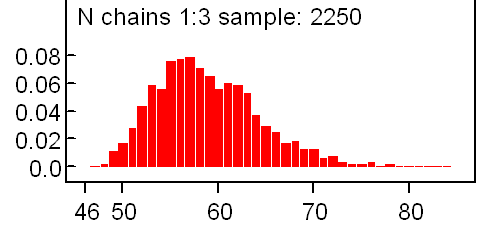
\includegraphics[width=3.5in]{Ch3/figs/Nchains}
\end{center}
\caption{Needs a caption}
\label{fig.nchains}
\end{figure}

\subsection{Extension of the Model}
One important issue in understanding the meaning of estimates produced under the individual covariate model  is that the uniform distribution on maxD implies that density is {\it not constant} over space. In particular, this model implies that it {\it decreases} as we move away from the centroid of the trap array. This is one reason we have a lower estimate of density than that obtained previously and also why, if we were to increase maxD, we would see density continue to decrease: $x[i] \sim \mbox{Uniform}(0,maxD)$ implies constant N in each distance band from the centroid but obviously the {\it area} of each distance band is increasing.  The reader can verify this as a homework exercise.
Obviously, the use of an individual covariate model is {\it not} restricted to use of this specific distribution for the individual covariate. Clearly, it is a bad choice and, therefore,  we should think about whether we can choose a better distribution for maxD - one that doesn't imply a decreasing density as distance from the centroid increases.  Conceptually, what we want to do is impose a prior on distance from the centroid, $x$, such that density is proportional to the amount of area in each successive distance band as you move farther away from the centroid.  In fact, there is theory that exists which tells us what the correct distribution of $x$ is $2x/maxD^2$. This can be derived by noting that $F(x) = Pr(X<x) = pi*x*x/pi*maxD*maxD$ . Then, $f(x) = dF/dx = 2*x/(maxD*maxD)$.  This might be called a triangular distribution, I think, which makes sense because the incremental area in each additional distance band increases linearly with radius (i.e., distance from centroid). It is sometimes comforting to verify things empirically:
\begin{verbatim}
> u<-runif(10000,-1,1)
> v<-runif(10000,-1,1)
> d<- sqrt(u*u+v*v)
> hist(d[d<1])
> hist(d[d<1],100)
> hist(d[d<1],100,probability=TRUE)
> abline(0,2)
\end{verbatim}

It would be useful if we could describe this distribution in *BUGS but there is not a built-in way to do this.  One possibility is to use a discrete version of the pdf. We might also be able to use what is referred to in WinBUGS jargon as the ``zeros trick'' (see Advanced BUGS tricks) although we haven't pursued this approach. Instead, we consider using a discrete version and break Dmax into L distance classes of width $\delta$, with probabilities proportional to $2*x$. In particular, if the cut-points are $xg[1]=0,xg[2], \ldots, xg[L+1]=Dmax$ and the interval midpoints are $xm[i] = xg[i+1]-\delta$. Then, the interval probabilities are $p[i] = 2*xm[i]*delta/(Dmax*Dmax)$, which we can compute once and then send them to WinBUGS as data.

The R script is as follows. In the model description the variable $x$ (observed home range center) has been rounded so that the discrete version of the $f(x)$ can be used as described previously. The new variable labeled \mbox{\tt xround} is actually then the integer category label in units of delta from 0. Thus, to convert back to distance in the expression for $lp[i]$, \mbox{\tt xround[i]} has to be multiplied by $\delta$.

\begin{verbatim}
delta<-.2
xround<-xcent%/%delta  + 1
Dgrid<- seq(delta,maxD,delta)
xprobs<- delta*(2*Dgrid/(maxD*maxD))
xprobs<-xprobs/sum(xprobs)

cat("
model{
p0 ~ dunif(0,1)       # prior distributions
mup<- log(p0/(1-p0))
psi~dunif(0,1)
beta~dnorm(0,.01)

for(i in 1:(nind+nz)){
  xround[i]~dcat(xprobs[])
  z[i]~dbern(psi)                     # zero inflation variables
  lp[i] <- mup + beta*xround[i]*delta # individual effect
  logit(p[i])<-lp[i]
  mu[i]<-z[i]*p[i]
  y[i]~dbin(mu[i],K)  #  observation model
 }

N<-sum(z[1:(nind+nz)])
}
",file="modelMcov.txt")
\end{verbatim}

To fit the model we do this - keeping in mind that the data objects required below have been defined in previous analyses of this chapter:

\begin{verbatim}
data2<-list(y=ytot,nz=nz,nind=nind,K=T,xround=xround,xprobs=xprobs,delta=delta)
params2<-list('p0','psi','N','beta')
inits =  function() {list(z=z, psi=psi, p0=runif(1),beta=rnorm(1) ) }
fit = bugs(data2, inits, params2, model.file="modelMcov.txt",working.directory=getwd(),
       debug=FALSE, n.chains=3, n.iter=11000, n.burnin=1000, n.thin=2)
\end{verbatim}

This is a useful model because it induces a clear definition of area in which the population of $N$ individuals reside. Under this model, that area is defined  by specification of maxD. We can apply the model for different values of maxD and observe that the estimated $N$ varies with $maxD$. Fortunately, we see empirically, that while N seems highly sensitive to the prescribed value of $maxD$, density seems to be invariant to $maxD$ as long as it is chosen to be sufficiently large. We fit the model for $maxD=12$ (points in close proximity to the trap arra)  to 20 for and the results are given in Table \ref{tab.xyz}.

\begin{table}
\caption{Table: Analysis of Fort Drum bear hair snare data using the individual covariate model, for different values of Dmax, the upper limit of the uniform distribution of `distance from centroid of the trap array' }
\begin{tabular}{cccc}
     maxD   mn    SD
[1,]  12 0.230 0.038
[2,]  15 0.244 0.041
[3,]  17 0.249 0.044
[4,]  18 0.249 0.043
[5,]  19 0.250 0.043
[6,]  20 0.250 0.044
\end{tabular}
\end{table}
%ANDY - I couldn't get this to show up right, I'll look into it if I
%get a chance


We see that the posterior mean and SD of density (individuals per square km) appear insensitive to choice of $maxD$ once we get a slight ways away from the maximum observed value of about 11.5. The estimated density of 0.250 per km$^2$ is actually quite a bit lower than we reported using model Mh (0.37, see section XYZ above) for which sample area is not an explicit feature of the model. On the other hand it is higher than that reported from Model M0 using the buffered area (0.195). There is no basis really for comparing or contrasting these various estimates and it would be a useful philosophical exercise for the reader to discuss this matter. In particular, application of model M0 and Mh are distinctly {\it not} spatially explicit models -- the area within which the population\footnote{We need to look back at Chapter 1 and make sure we quit calling this ``sample area'' - it really isn't that at al, but rather the area within which N resides.} resides is not defined under either model. There is therefore no reason at all to think that the estimates produced under either model, using a buffered area, are justifiable based on any theory. In fact, we would get exactly the same estimate of $N$ no matter what we declare the area to be. On the other hand, the individual covariate model explicitly describes a distribution for ``distance from centroid'' that is a reasonable and standard null model - it posits, in the absence of direct information, that individual home range centers are randomly distributed in space and that probability of detection depends on the distance between home range center and the centroid of the trap array. Under this definition of the system, we see that density is invariant to the choice of sample area which seems like a desirable feature. The individual covariate model is not ideal, however, because it does not make full use of the spatial information in the data set, i.e., the trap locations and the locations of each individual encounter.


\subsection{Invariance of density to maxD}

Under the model above, and also under models that we consider in later chapters, a general property of the estimators is that while N increases with the prescribed trap area (equivalent to maxD in this case), we expect that density estimators should be invariant to this area. In the model used above, we note that
$Area(maxD) = \pi*maxD*maxD$ and $E[N(maxD)] = \lambda*A(maxD)$ and thus $E[Density(maxD)] = \lambda$  which is constant. This should be interpreted as the {\it prior} density. Absent data, then realizations under the model will have density $\lambda$ regardless of what $maxD$ is prescribed to be.  As we verified empirically above, the posterior density is also invariant if $maxD$ as long as the implied area (implied by maxD) is large enough so that the data no longer provide information about density (i.e., ``far away''), then our estimator of density should become insensitive.

\subsection{Toward Fully Spatial Capture-recapture Models}
We developed this model for the average observed location and equated it to home range center $s_{i}$. Intuitively, taking the average encounter location as an estimate of home range center makes sense but more so when the trapping grid is dense and expansive relative to typical home range sizes.  However, our approach also ignored  the variable precision with which each $s[i]$ is estimated and also, as noted previously, estimates of $s[i]$ around the ``edge'' (however we define that) are biased because the observations are truncated (we can only observe locations within the trap array).  In the next Chapter we provide a further extension of this individual covariate model that definitively resolves the ad hoc nature of the individual covariate approach we took here. In that model we build a model in which $s[i]$ are regarded as latent variables and the observation locations (i.e., trap specific encounters) are linked to those latent variables with an explicit model. We note that the model fitted previously could be adapted easily to deal with $s_{i}$ as a latent variable, simply by adding a prior distribution for $s_{i}$. The reader should contemplate how to do this in WinBUGS.


\section{DISTANCE SAMPLING: A primative Spatial Capture-Recapture Model}

Distance sampling is one of the most popular methods for estimating
animal abundance. One of the great benefits of distance sampling is
that it provides explicit estimates of {\it density}. The distance
sampling model is a special case of a closed population model with a
covariate. The covariate in this case, $x_{i}$, is the distance
between an individual's location ``$u$'' and the observation location
or transect. In fact, the model underlying distance sampling is
precisely the same model as that which applies to the
individual-covariate models, except that observations are made at only
$K=1$ sampling occasion. In a sense, distance sampling is a spatial
capture-recapture model, but without the ``recapture.''  This first
and most basic spatial capture-recapture model has been used routinely
for decades and, formally, it is a spatially-explicit model in the
sense that it describes, explicitly, the spatial organization of
individual locations (although this is not always stated explicitly)
and, as a result, somewhat general models of how individuals are
distributed in space can be specified \citep{royle_etal:2004,
  johnson_etal:2010, sillett_etal:2011}.
As before, the distance sampling model, under data augmentation, includes a set of $M$ zero-inflation variables $z_{i}$ and the binomial model expressed conditional on $z$ (binomial for $z=1$, and fixed zeros for $z=0$).  In distance sampling we pay for having only a single sample (i.e., $K=1$) by requiring constraints on the model of detection probability. A standard model is
\[
\log(p_{i}) = b * x_{i}^{2}
\]
for $b < 0$, where $x_i$ denotes the distance at which the $i$th
individual is detected relative to some reference location where
perfect detectability ($p=1$) is assumed. This function corresponds to
the ``half-normal'' detection function (i.e., with $b =
1/\sigma^{2}$).  If $K>1$ then the intercept alpha is identifiable and
such models are usually called ``capture-recapture distance
sampling''\citep{borchers_etal:XXXX} and others XYZ????).

As with previous examples, we require a distribution for the individual covariate $x_{i}$. The customary choice is
\[
x_{i} \sim \mbox{Uniform}(0,B)
\]
wherein $B>0$ is a known constant, being the upper limit of data
recording by the observer (i.e., the point count radius, or transect
half-width). In practice, this is sometimes asserted to be infinity,
but in such cases the distance data are usually truncated.
Specification of this distance sampling model in the BUGS language is
shown in Panel \ref{panel.distance}. \citet{royle_dorazio:2008}, p. xyz) provide a distance sampling example analyzed by DA using the famous Impala data.


\begin{panel}[htp]
\centering
\rule[0.15in]{\textwidth}{.03in}
\begin{minipage}{5in}
\begin{verbatim}
b~dunif(0,10)
psi~dunif(0,1)

for(i in 1:(nind+nz)){
   z[i]~dbern(psi)    # DA Variables
   x[i]~dunif(0,B)    # B=strip width
   p[i]<-exp(logp[i])   # DETECTION MODEL
   logp[i]<-   -((x[i]*x[i])*b)
   mu[i]<-z[i]*p[i]
   y[i]~dbern(mu[i])  # OBSERVATION MODEL
 }
N<-sum(z[1:(nind+nz)])
D<- N/striparea  # area of transects
\end{verbatim}
\end{minipage}
\rule[-0.15in]{\textwidth}{.03in}
\caption{Distance sampling model in WinBUGS, using a ``half-normal''
detection function.}
\label{panel.distance}
\end{panel}


As with the individual covariate model in the previous section, the distance sampling model can be equivalently specified by putting a prior distribution on individual {\it location} instead of distance between individual and observation point (or transect).
Thus we can write the general distance sampling model as
\[
 logit(p[i]) = alpha + beta*||u[i] - x0||
\]
Along with
\[
 {\bf u}_{i} \sim Uniform({\cal S})
\]
where $x_{0}$ is a fixed point (or line) and $u[i]$ is the individual's location which is observable for n individuals. In practice it is easier to record distance instead of location.  Basic math can be used to argue that if individuals have a uniform distribution in space, then the distribution of Euclidean distance is also uniform. In particular, if a transect of length L is used and x is distance to the transect then $F(x) = Pr(X<=x) = L*x/L*B = x/B$ and $f(x) = dF/dx = (1/B)$. For measurements of radial distance, see the previous section.

In the context of our general characterization of SCR models (chapter 1.XYZ), we suggested that every SCR model can be described, conceptually, by a hierarchical model of the form:
\[
 [y|u][u|s][s].
\]
Distance sampling ignores $s$, and treats u as observed data\footnote{Formally we could also say that $[u] = \int [y|s][s] ds$}. Thus, we are left with
\[
[y|u][u].
\]
In contrast, as we will see in the next chapters, basic SCR models (chapter 4) ignore $u$ and condition on $s$, which is not observed:
\[
[y|s][s]
\]
Since $[u]$ and $[s]$ are both assumed to be uniformly distributed, these are structurally equivalent  models! The main  differences have to do with interpretation of model components and whether or not the latent variables are observable (in distance sampling they are).

So why bother with SCR models when distance sampling yields density estimates and accounts for spatial  heterogeneity in detection? For one, imagine try to collect distance sampling data on tigers! Clearly, distance sampling requires that one can collect large quantities of distance data, which is not always possible. For tigers, it is much easier, efficient, and safer to employ camera traps or tracking plates and then apply SCR models. Furthermore, as we will see in Ch XYZ, SCR models can use distance data to estimate all the parameters of our enchilada, allowing us to study distribution, movement, and density. Thus, SCR models are much more flexible than distance sampling models, and can accommodate data from virtually all animal survey designs.


\subsection{Example: Muntjac deer survey from Nagarahole, India }
Here we fit distance sampling models to distance sampling data on the muntjac deer (Muntiakus muntjak) collected in the year 2004 from Nagarahole National Park in southern India \citep{kumar_etal:XXXX}(Kumar et al. unpublished data). The muntjac is a solitary species and distance measurements were made on 57 groups that were largely singletons with XYZ pairs of individuals.  Commands for reading in and organizing the data for WinBUGS, followed by writing the model to a text file. Note that the total sampled area of the transects is fed in as ``striparea'' which is 708 (km of transect) multiplied by the strip width (B=150 = 0.15 km) multiplied by 2.
\begin{verbatim}
library("R2WinBUGS")
data<- read.csv("Muntjac.csv")
nind<-nrow(data)
y<-rep(1,nind)
nz<-400
y<-c(y,rep(0,nz))
x<-data[,3]
x<-c(x,rep(NA,nz))
z<-y
data<-list(y=y,x=x,nz=nz,nind=nind,B=150,striparea=708*.15*2)

cat("
model{
b~dunif(0,10)
psi~dunif(0,1)

for(i in 1:(nind+nz)){
   z[i]~dbern(psi)    # DA Variables
   x[i]~dunif(0,B)    # B=strip width
   p[i]<-exp(logp[i])   # DETECTION MODEL
   logp[i]<-   -((x[i]*x[i])*b)
   #logp[i]<- -b*log(x[i]+1)
   mu[i]<-z[i]*p[i]
   y[i]~dbern(mu[i])  # OBSERVATION MODEL
 }
N<-sum(z[1:(nind+nz)])
D<- N/striparea  # area of transects
}
",file="dsamp.txt")
\end{verbatim}

Next, we provide inits, indicate which parameters to monitor, and then pass those things to WinBUGS:
\begin{verbatim}
params<-list('b','N','D','psi')
inits =  function() {list(z=z, psi=runif(1), b=runif(1,0,.02) )}
fit = bugs(data, inits,  params, model.file="dsamp.txt",
working.directory=getwd(),debug=T, n.chains=3, n.iter=4000, n.burnin=1000, n.thin=2)
\end{verbatim}
Posterior summaries are provided in the following table. Estimated density is pretty low, 1.1 individuals per sq. km.\footnote{ much lower than Samba's : Observers walked about 708 km from 39 transects in Nagarahole and the muntjac density is about 3 per sq km.. I need to get to the bottom of this.}
\begin{verbatim}
 node	 mean	 sd	 MC error	2.5%	median	97.5%	start	sample
D	1.096	0.1694	0.009122	0.8098	1.078	1.474	501	4500
N	232.8	35.99	1.938	172.0	229.0	313.0	501	4500
b	5.678E-4	1.05E-4	4.129E-6	3.867E-4	5.616E-4	7.949E-4	501	4500
deviance	681.2	16.72	0.7536	650.8	680.6	716.6	501	4500
psi	0.5099	0.08238	0.004442	0.3681	0.5033	0.6918	501	4500
\end{verbatim}


\section{Summary and Outlook}

Traditional closed population capture-recapture models are closely related to binomial generalized linear models.  Indeed, the only real distinction is that in capture-recapture models, the population size parameter $N$ (corresponding also to the size of a hypothetical ``complete'' data set) is unknown.  This requires special consideration in the analysis of capture-recapture models. The classical approach to inference recognizes that the observations don't have a standard binomial distribution but, rather, a truncated binomial (from which which the so-called ``conditional likelihood'' derives) since we only have encounter frequency data on observed individuals. If instead we analyze the models using data augmentation, the observations can be modeled using a zero-inflated binomial distribution. In short, when we deal with the unknown-N problem using data augmentation then we are left with zero-inflated GLM and GLMMs instead of ordinary GLM or GLMMs. The analysis of such zero-inflated models is practically convenient, especially using the various Bayesian analysis packages that use the BUGS language.

Spatial capture-recapture models that we will consider in the rest of the chapters of this book are closely related to what have been called individual covariate models. Heuristically, spatial capture-recapture models arise by defining individual covariates based on observed locations of individuals -- we can think of using some function of mean encounter location as an individual covariate. We did this in a novel way, by using distance to the centroid of the trapping array as a covariate. We analyzed the ``full likelihood'' using data augmentation, and placed a prior distribution on the individual covariate which was derived from an assumption that individual locations are, a priori, uniformly distributed in space. This assumption provides for invariance of the density estimator to the choice of population size area (induced by maximum distance from the centroid of the). The model addressed some important problems in the use of closed population models: it allows for heterogeneity in encounter probability due to the spatial context of the problem and it also provides a direct estimate of density because area is a feature of the model (via the prior on the individual covariate). The model is still not completely general because the model does not make use of the fully spatial encounter histories, which provide direct information about the locations and density of individuals.
A specific individual covariate model that is in widespread use is
classical ``distance sampling.'' The model underlying distance sampling is precisely a special kind of SCR model - but one without replicate samples. Understanding distance sampling and individual covariate models more broadly provides a solid basis for understanding and analyzing spatial capture-recapture models.

